\documentclass[11pt,a4paper]{article}

% Basic packages
\usepackage[fontset=fandol]{ctex}
\usepackage{amsmath, amssymb}
\usepackage{graphicx}
\usepackage[margin=2.15cm]{geometry}
\usepackage[most]{tcolorbox}
\usepackage{etoolbox}
\usepackage{listings}
\usepackage{hyperref}
\usepackage{booktabs}
\usepackage{subcaption}
\usepackage{float}
\usepackage{tikz}
\IfFileExists{pgfplots.sty}{
    \usepackage{pgfplots}
    \pgfplotsset{compat=1.18}
}{}

% Highlight box palette: low-saturation and print-friendly.
% Visual weight is ordered by teaching role, so a page mixing several boxes still
% reads important > warning > knowledge > dialogue instead of competing for attention.
% Title text is white on every title bar; contrast stays within WCAG AA (4.5:1--6.0:1).
\definecolor{kbBack}{HTML}{F2F6FA}\definecolor{kbFrame}{HTML}{9DB4CC}\definecolor{kbTitle}{HTML}{52708F}
\definecolor{ibBack}{HTML}{FBF5E7}\definecolor{ibFrame}{HTML}{C9A961}\definecolor{ibTitle}{HTML}{7D5F1E}
\definecolor{wbBack}{HTML}{FCF2F0}\definecolor{wbFrame}{HTML}{D6A096}\definecolor{wbTitle}{HTML}{9E4F43}
\definecolor{dbBack}{HTML}{F4F7F3}\definecolor{dbFrame}{HTML}{AEC2AC}\definecolor{dbTitle}{HTML}{5F7F64}

\tcbset{softbox/.style={
    enhanced, boxrule=0.8pt, arc=2pt, left=3mm, right=3mm, top=2mm, bottom=2mm,
    coltitle=white, fonttitle=\bfseries, toptitle=0.6mm, bottomtitle=0.6mm
}}

% Highlight boxes
\newtcolorbox{knowledgebox}[1]{
    softbox, colback=kbBack, colframe=kbFrame, colbacktitle=kbTitle, title=#1
}

\newtcolorbox{importantbox}[1]{
    softbox, colback=ibBack, colframe=ibFrame, colbacktitle=ibTitle, title=#1
}

\newtcolorbox{warningbox}[1]{
    softbox, colback=wbBack, colframe=wbFrame, colbacktitle=wbTitle, title=#1
}

\newtcolorbox{dialoguebox}[1]{
    softbox, breakable, colback=dbBack, colframe=dbFrame, colbacktitle=dbTitle, title=#1
}

% Listings
\lstset{
    language=Python,
    basicstyle=\ttfamily\small,
    keywordstyle=\color{blue},
    stringstyle=\color{red!60!black},
    commentstyle=\color{green!60!black},
    breaklines=true,
    frame=single,
    numbers=left,
    numberstyle=\tiny\color{gray},
    captionpos=b,
    extendedchars=false
}

\usepackage{tabularx}
\newcolumntype{L}[1]{>{\raggedright\arraybackslash}p{#1}}
\hypersetup{colorlinks=true,linkcolor=kbTitle,urlcolor=kbTitle,pdftitle={CMU L6 编程与软件开发 Agent：中文课程讲义},pdfauthor={Based on Graham Neubig; Chinese notes prepared with Codex}}
\renewcommand{\baselinestretch}{1.13}
\setlength{\parskip}{.4em}
\setlength{\emergencystretch}{2em}
\setcounter{tocdepth}{1}
\captionsetup{font=small,labelfont=bf}
\lstset{basicstyle=\ttfamily\footnotesize,columns=fullflexible,keepspaces=true,xleftmargin=6mm,framexleftmargin=4mm}
\begin{document}
\special{pdf:minorversion 7}
\hypersetup{pageanchor=false}
\begin{titlepage}
\centering
\vspace*{.9cm}
{\Large CMU 11-768 · AI Agents\par}
\vspace{.6cm}
{\Huge\bfseries 编程与软件开发 Agent\par}
\vspace{.4cm}
{\Large 从代码模型到可验证的软件开发流程\par}
\vspace{.5cm}
{\large L6 中文课程讲义\par}
\vspace{1cm}
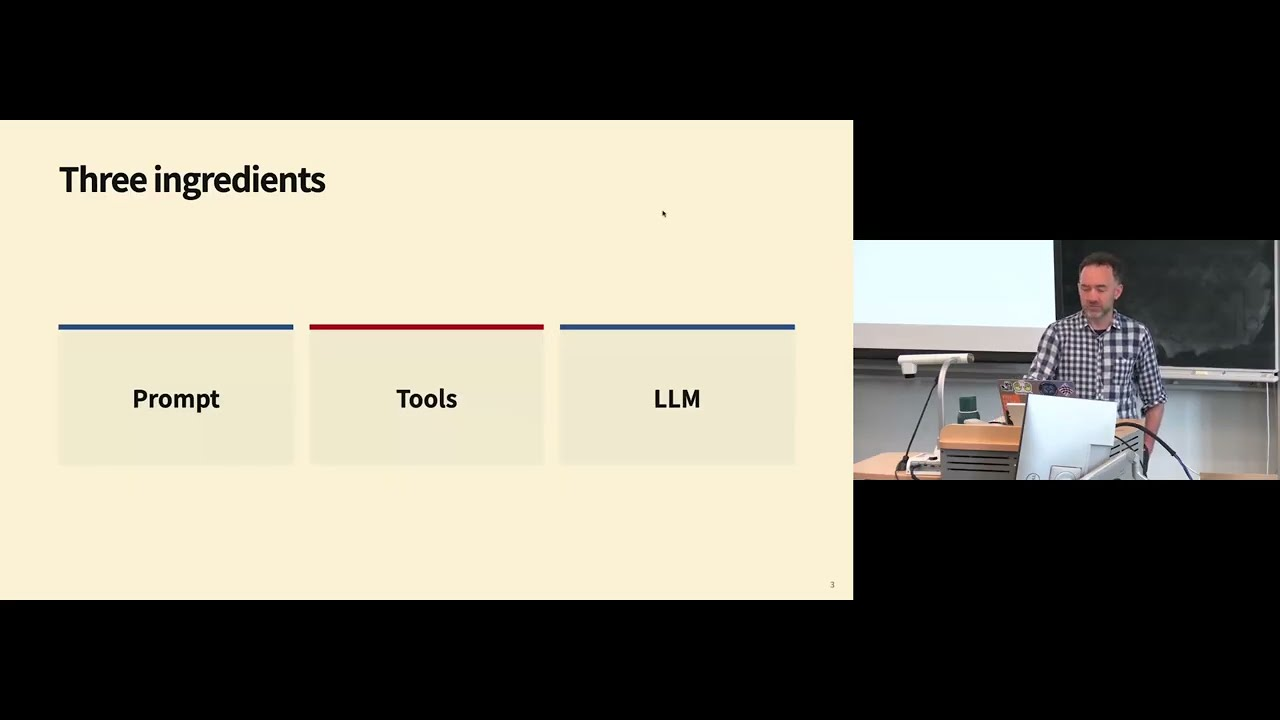
\includegraphics[width=\textwidth]{figures/原视频封面.jpg}\par
{\small 图：原视频封面\par}
\vfill
\begin{tcolorbox}[colback=kbBack,colframe=kbFrame,width=\textwidth]
\textbf{主讲 / 频道}：Graham Neubig\par
\textbf{课程}：Carnegie Mellon University，11-768 AI Agents，Fall 2026\par
\textbf{时长}：78 分 49 秒\par
\textbf{整理日期}：2026 年 10 月 3 日\par
\textbf{原视频}：\href{https://www.youtube.com/watch?v=1BWeH1oOM7k}{youtube.com/watch?v=1BWeH1oOM7k}
\end{tcolorbox}
\end{titlepage}
\pagenumbering{arabic}
\hypersetup{pageanchor=true}
\section*{本讲概览}
编程 Agent 需要一套相互配合的能力：模型理解代码与修改意图，工具让它访问和改变仓库，环境反馈让它检查修改后的行为。本讲从单步代码模型的训练和评价出发，展开定位、编辑、验证的循环，再进入可执行训练任务、前端验证以及维护、测试与 CI 等软件开发工作。

讲义依据带时间课程转录与 82 页官方课件整理，并结合原始资料核对机制。图示采用官方课件矢量裁图，图注注明官方 PDF 页码与对应口述区间。代码节选和教学示例分别说明用途，实验数值保留各自的评测条件。课程末尾因时间限制未展开的代码行为预测，作为明确标注的课件补充单独介绍。
材料入口：\href{https://www.cmu-agents.com/slides/lecture-06-coding-agents.pdf}{官方课件}；\href{https://www.usetranscribe.io/yt/1BWeH1oOM7k/coding-agents-software}{带时间课程转录}。各章提供相关原始研究链接。
\tableofcontents
\clearpage
\section{从写一段代码到参与软件开发}
\subsection{三种任务尺度}
“会写代码”可以指三个范围差别很大的任务。第一种是根据一个相对完整的提示生成代码，例如给定 CSV 数据与绘图要求，输出创建柱状图的程序。第二种是在已有仓库中修复问题或实现功能，修改可能横跨多个文件。第三种是参与软件开发过程，包含维护、测试、评审与构建等工作。课程沿着这三种尺度展开，先解释代码模型如何形成能力，再讨论工具与工作流程。

\begin{center}
\small
\begin{tabularx}{\textwidth}{L{2.4cm}XX}
\toprule
任务尺度 & 主要输入与产物 & 关键困难 \\
\midrule
单步代码生成 & 需求描述、数据或函数签名；输出一段代码 & 理解规格，选择算法，写出可运行的实现 \\
仓库级修改 & Issue、已有文件与依赖；输出跨文件修改 & 找到相关位置，保留既有行为，验证修改 \\
软件开发过程 & 代码、测试、构建与协作记录；推动开发任务完成 & 处理多种反馈，满足功能与质量要求 \\
\bottomrule
\end{tabularx}
\end{center}

这三种任务都依赖\textbf{提示、工具与语言模型}。提示表达目标和限制；工具让 Agent 搜索、编辑和执行；模型决定怎样理解问题、选择下一步并形成修改。本讲将主要篇幅放在后两项，提示中的长上下文、技能与记忆则与此前课程相接。

\begin{importantbox}{代码模型与编程 Agent 的能力边界}
一次调用生成程序，展示的是模型的代码生成能力。让模型查看仓库、执行工具、读取结果并继续修改，才形成带环境反馈的 Agent 循环。因此，单步生成成绩与完整开发任务成绩回答的是不同问题。
\end{importantbox}

\subsection{代码模型需要哪些能力}
即使暂时不调用工具，一个代码模型也要同时掌握三类能力。
\begin{itemize}
\item \textbf{编程语言知识}：语法、API、惯用写法与库的用法。知道某个函数名还不够，还要知道参数、返回值及适用条件。
\item \textbf{编辑能力}：根据空缺两侧的内容修改已有代码。开发者通常持续修改程序，编辑场景中的右侧上下文包含重要约束。
\item \textbf{推理能力}：把自然语言规格转成程序行为，选择算法，检查边界情况。代码和数学适合研究推理模型的一项原因，是许多结果可以通过执行或其他检查获得反馈。
\end{itemize}

这些能力需要相应的数据和训练设计。训练语料包含代码，并不自动保证模型能在文件中间编辑；能补全语法，也不自动保证模型理解复杂需求或跨文件依赖。

\subsection{训练路线：基础知识、定向适配与反馈优化}
课程将代码模型的形成分为三个阶段。
\begin{center}
\small
\begin{tabularx}{\textwidth}{L{2.5cm}XX}
\toprule
阶段 & 主要训练材料或信号 & 希望形成的能力 \\
\midrule
预训练 & 大规模代码、自然语言、技术说明和数学语料 & 语言与代码的基础规律，文本与代码之间的联系 \\
中期训练 & 增加代码比例，组织较长的相关代码序列，引入编辑任务 & 更强的代码专长、长上下文与编辑能力 \\
RL 后训练 & 推理与最终程序，执行得到的奖励 & 提高任务成功率，学习利用可验证反馈 \\
\bottomrule
\end{tabularx}
\end{center}

讲者在本讲中把持续预训练、部分定向适配和监督微调放在较宽泛的“中期训练”讨论里。这是一种讲课组织方式：实际方案中，它们使用的数据形式和优化目标可以不同。后文先讲代码领域需要特别处理的事项，再展开执行评价与奖励；通用监督微调和 RL 算法的完整推导留给后续课程。

\subsection{本章小结}
编程任务可以从单步生成扩展到仓库修改和整个开发过程。要理解编程 Agent，先区分模型的语言、编辑与推理能力，再观察工具如何把这些能力接入真实环境。训练路线中的语料、上下文组织与奖励信号，分别决定模型能看到什么、能联系什么以及什么结果会受到强化。

\clearpage
\section{代码预训练：数据结构与 Token 表示}
\subsection{为什么训练数据必须同时包含代码与说明}
用户经常用自然语言提出需求，模型却需要输出程序。只看源码，模型获得的需求解释、技术说明与代码之间的关联会不足。因此，课程列出网页文本、技术文章、数学、源码和文档等来源。尤其有价值的是解释和实现相邻出现的材料，例如教程中先说明 API，再给出调用代码。

基础训练通常仍然采用下一 Token 预测：给定之前的内容，提高真实下一项出现的概率。对整个混合语料求平均后，得到课件中的语言模型损失。
$$
\mathcal{L}_{\mathrm{LM}}
=-\mathbb{E}_{x\sim D_{\mathrm{mix}}}
\left[\sum_{t=1}^{|x|}\log p_\theta(x_t\mid x_{<t})\right].
$$
\begin{itemize}
\item $\mathcal{L}_{\mathrm{LM}}$：语言模型训练的负对数似然损失。
\item $D_{\mathrm{mix}}$：由代码、文本等来源组成的训练数据分布。
\item $x$：从该分布取出的一个 Token 序列；$|x|$ 是它的长度。
\item $t$：序列中的位置；$x_t$ 是该位置的真实 Token，$x_{<t}$ 是此前所有 Token。
\item $p_\theta$：参数为 $\theta$ 的模型给出的条件概率。
\item $\mathbb{E}$：对训练样本求期望；$\sum$ 将各位置的损失相加；$\log$ 为对数。
\end{itemize}

同样的预测目标，在不同的数据组织下可以学到不同东西。Python 的缩进决定代码块归属，不能沿用把连续空格压成一个空格的普通文本清洗方式。文件边界、API 名称与 Markdown 中的代码块，也应保持可识别的结构。训练时除观察各领域的留出损失，还应运行功能性代码任务：较低预测损失与任务成功率需要分别检查。

\begin{importantbox}{代码结构属于训练信息}
缩进、换行、文件边界以及说明与代码的对应关系，都会影响程序的解释。清洗的目标是提高数据质量，同时保存这些信息。删除结构之后，增加语料规模也无法补回被删除的关系。
\end{importantbox}

\subsection{选择、去重、来源记录与评测去污染}
公开代码并不是均匀分布的。一个流行项目可能有成千上万的 fork；依赖库可能被复制进大量仓库；生成代码和重复解答也可能占据很大比例。直接累积下载量，会让重复内容挤占训练预算。

课程将数据处理拆成四件事，各自解决一个问题。
\begin{enumerate}
\item \textbf{按语言与来源过滤}：剔除损坏编码、低价值重复和不适合训练目标的生成文件。这里针对的是数据质量；“由程序生成”本身并不是所有场景下的淘汰理由。
\item \textbf{去重}：识别 fork、仓库内附带的第三方库、近似相同的文件以及复制的题解，减少同一内容的反复采样。
\item \textbf{保留来源信息}：记录许可证、采集日期、退出请求与敏感信息过滤情况。源代码中可能包含密钥；课程提及使用自动扫描工具识别这些内容。
\item \textbf{控制训练与评价的交叠}：按仓库或问题家族划分数据，并检查评测任务是否出现在训练材料里。否则，模型可能在评价时复现见过的题目，成绩就难以说明对新问题的能力。
\end{enumerate}

\begin{warningbox}{只随机划分文件，仍可能泄漏}
若同一仓库的 fork 或近似副本分别进入训练集和测试集，文件名不同也不能消除内容重叠。去重与划分应考虑代码的来源和相似关系；评测去污染还要单独检查题目与解答。
\end{warningbox}

StarCoder 是本段主要的公开实例。它不仅使用源码，也纳入 issues、commits 和 notebooks。理解训练集时，需要同时问：材料从哪里来、怎样清洗，以及它能提供什么任务信号。

\subsection{Tokenizer：保存空白，同时压缩常见模式}
代码 Token 不等于编程语言词法分析器中的词法单元。一个标识符可以分成多个子词；一个 Token 也可以覆盖换行和若干空格。课程采用字节级 BPE 说明这件事：通过合并常见字节序列得到词表，既要保存原始内容，也要避免每个空格都耗费一个 Token。

\begin{figure}[H]
\centering
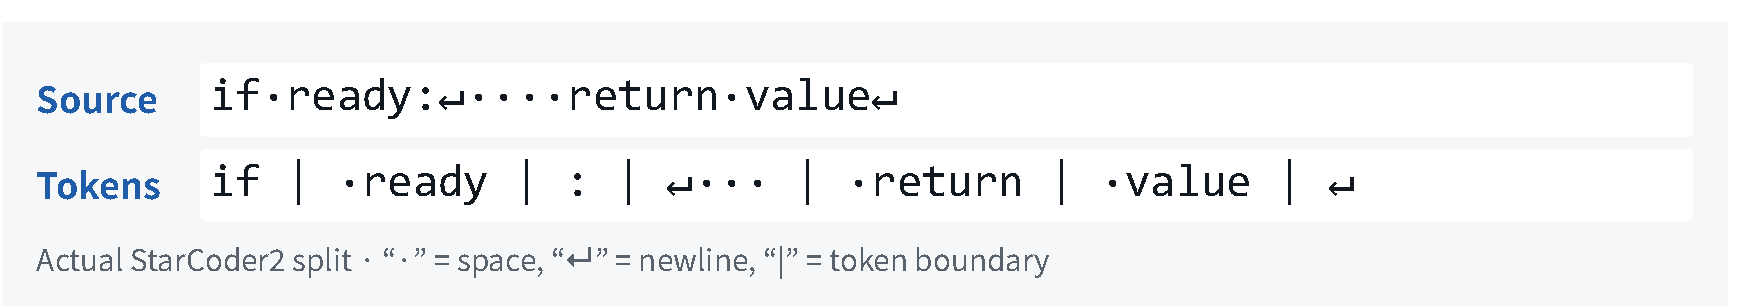
\includegraphics[width=\textwidth]{figures/代码空白与子词切分.pdf}
\caption{课件用 StarCoder2 的真实切分展示空白如何并入 Token。圆点表示空格，回车箭头表示换行，竖线表示 Token 边界。来源：官方课件第 9 页；对应口述 00:11:54--00:19:15。}
\end{figure}

图中的原文包含换行后四个空格。切分后，换行加前三个空格形成一项，第四个空格随 \texttt{return} 进入下一项。这种切分保留全部字符，同时减少空白占用的 Token 数。它没有把 Python 的缩进改成三个空格。

课堂讨论进一步指出：BPE 的合并规则原则上可以跨越空白边界。更长的合并片段能缩短表示，但会给部分前缀补全带来麻烦。例如，若一段常用 import 语句被合成过大的单元，编辑器中的光标可能停在这个单元内部，补全就需要处理 Token 边界与字符边界不一致的问题。词表设计因此同时影响长度效率与编辑行为；不能只比较压缩率。

\begin{knowledgebox}{空白的两个角色}
空格、制表符和换行在一些语言中决定语法，在字符串字面量中也可能决定内容。将常见空白序列合并成 Token，仍然能够保存这些字符；将它们从原文删除或归一化，则会改变程序。
\end{knowledgebox}

\subsection{多语言能力与默认语言倾向}
StarCoderBase 的课堂实例是 15.5B 参数、1T 训练 Token、80 余种编程语言。图中横轴为已经训练的 Token 数，单位为十亿；纵轴为单次生成的测试通过率 pass@1；每条曲线对应一种编程语言。多数语言随训练推进改善，但不同语言的水平和变化幅度并不相同。

\begin{figure}[H]
\centering
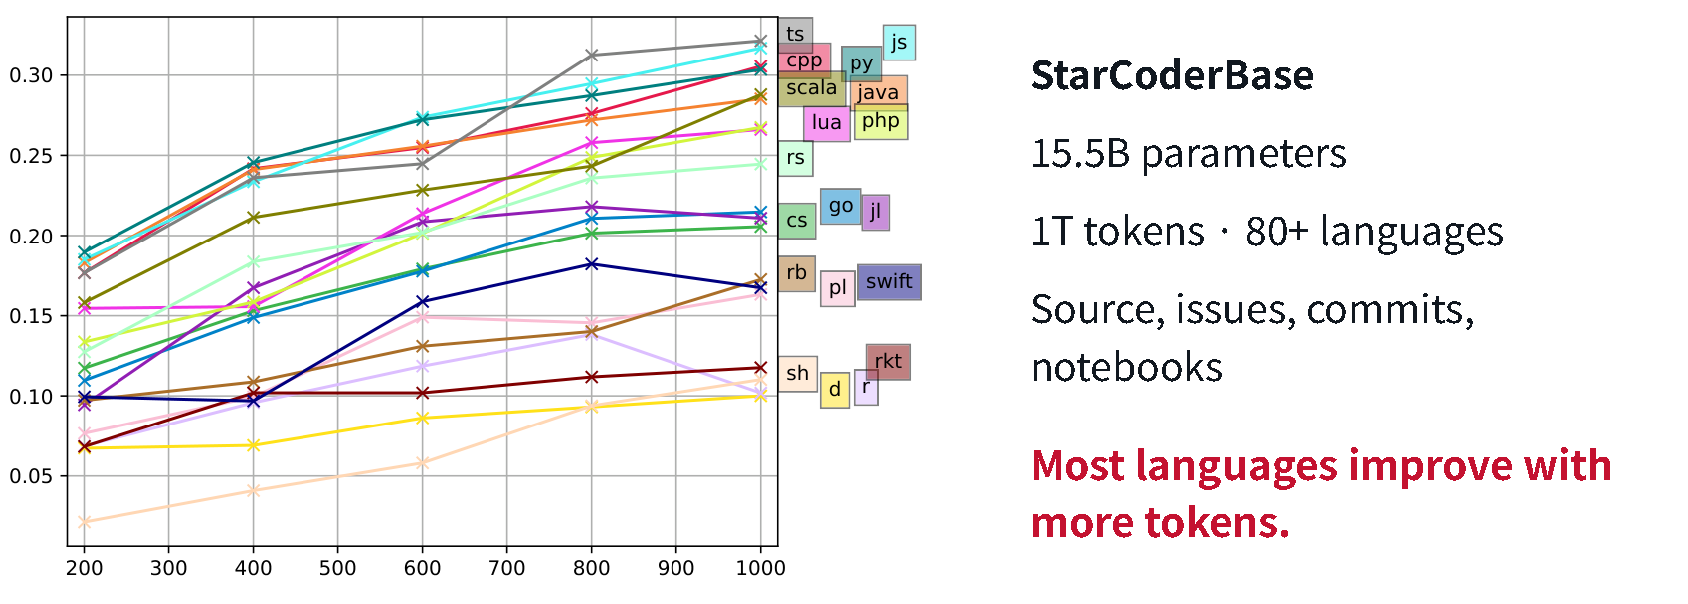
\includegraphics[width=\textwidth]{figures/StarCoder多语言训练曲线.pdf}
\caption{多语言代码能力随训练推进变化，语言之间存在明显差异。该图是 StarCoder 研究的训练结果。来源：官方课件第 10 页；对应口述 00:14:16--00:16:58。}
\end{figure}

能力差异还会反映为语言选择的倾向。讲者举例：没有明确指定语言时，他经常看到数据处理任务用 Python，界面任务使用 React；在把数据处理程序迁移到 Rust 后，后续生成仍会回到 Python，需要再次强调目标语言。这是课堂经验，而非所有模型的固定规则。讲者提出的可能原因包括语料中的流行程度、语言书写的便利，以及后训练中实际可用的执行器。

因此，评价代码模型时既要看指定语言的正确率，也要看模型能否持续遵守语言与环境要求。支持某种语言、擅长该语言以及在未指定时选择该语言，是三个不同属性。

\subsection{本章小结}
代码预训练采用通用预测目标，但数据必须保留程序结构和文本与代码的联系。过滤、去重、来源记录与评测去污染决定训练预算和评价是否有意义。Tokenizer 在字符保真、表示长度与编辑边界之间做取舍；多语言语料和执行环境则影响模型的能力分布与默认选择。

\subsection{拓展阅读}
\begin{itemize}
\item \href{https://arxiv.org/abs/2305.06161}{StarCoder: may the source be with you!}：公开代码语料、过滤、去重、Token 化及多语言评价。
\item \href{https://arxiv.org/abs/2402.00838}{OLMo}：可供对照的数据、训练与评价公开方案。
\end{itemize}

\clearpage
\section{定向适配：长上下文、Infilling 与开发信号}
\subsection{增加代码比例，同时保留理解需求的能力}
具备一般语言能力的模型，可以继续训练为更强的代码模型。Code Llama 的课件实例从 Llama 2 权重出发，为 7B、13B、34B 模型继续训练 500B Token。这里的 B 表示十亿；这组数字描述该研究的训练规模。

增加代码比例的同时，还要测量数学和通用语言能力是否退化。课程引用 Qwen2.5-Coder 的数据混合消融。下表重排了选定列，纯代码训练与 70\% 代码、20\% 文本、10\% 数学的混合训练相比，代码得分变化较小，数学和通用问答得分则明显改善。

\begin{table}[H]
\centering
\small
\begin{tabular}{lrrr}
\toprule
代码 / 文本 / 数学比例 & Common code & MATH & MMLU \\
\midrule
100 / 0 / 0 & 49.8 & 10.3 & 42.8 \\
70 / 20 / 10 & 48.3 & 33.2 & 62.9 \\
\bottomrule
\end{tabular}
\caption{Qwen2.5-Coder 数据混合实验的选定列。官方课件第 12 页将纯代码组的 MMLU 写成 23.8；这里按原论文 Table 3 更正为 42.8，23.8 实为该组的 GSM8K 得分。对应口述 00:19:15--00:21:06。}
\end{table}

这组结果说明了一个训练目标：保留解释需求和推理所需的基础能力，同时加强代码专长。它并没有给出所有模型都应使用的固定比例。混合比例需要在同一训练方案中做实验，并同时观察代码、数学和通用任务。

\subsection{长上下文训练要提供有联系的文件}
仓库级修改需要理解分散在不同文件中的约束。把整个仓库直接拼起来是一个朴素办法，但大仓库常常超出上下文预算，且其中大量文件与当前任务无关。课程建议构造连贯的训练序列：同一目录的相关文件，或沿依赖图收集的文件，配上文件路径与边界。

\begin{figure}[H]
\centering
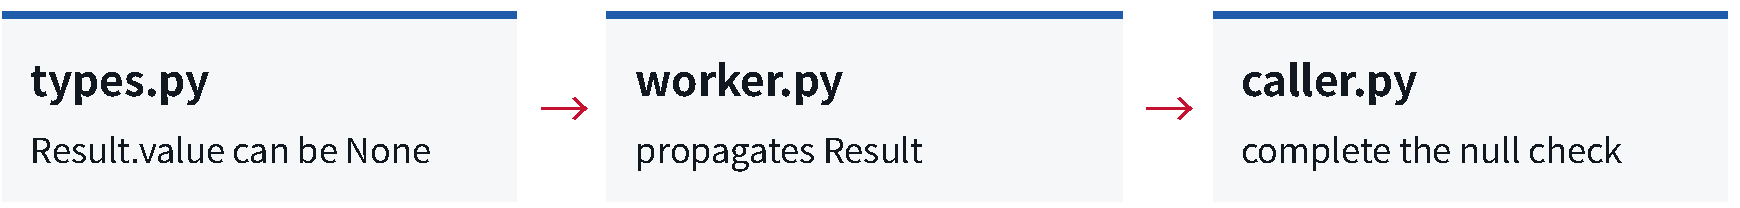
\includegraphics[width=\textwidth]{figures/跨文件依赖与空值检查.pdf}
\caption{调用端的空值检查依赖类型定义和中间文件的信息，体现跨文件上下文的用途。来源：官方课件第 13 页；对应口述 00:21:06--00:22:57。}
\end{figure}

图中的 \texttt{types.py} 说明 \texttt{Result.value} 可以是 \texttt{None}；\texttt{worker.py} 传递这个对象；\texttt{caller.py} 的补全应尊重前面给出的约束。如果训练序列只包含调用端，模型很难学习到这种跨文件联系。

Qwen2.5-Coder 的课件实例采用 8K 到 32K 的训练长度扩展，再通过 YaRN 支持 128K。长序列数据和位置处理要共同配合；验证时应检查跨文件补全、文件中间补全，以及原有短上下文能力是否保留。这个思路与 L3 的长上下文建模直接相接：扩大可容纳长度之后，还需要让模型学会使用其中的依赖关系。

\subsection{Infilling：缺口右侧也是输入}
开发者常常在已有程序内部修改一小段。以返回类型为例，若光标停在类型注解处，普通从左向右的补全只看到函数签名；缺口后面的函数体则直接提供返回值的信息。课件用下面的函数说明这一点。代码是课件示例的可运行版本。

\par\noindent\begin{minipage}{\textwidth}
\begin{lstlisting}[caption={根据缺口后的函数体补出 bool 返回类型（课件示例）}]
def is_positive(x: int) -> bool:
    return x > 0
\end{lstlisting}
\end{minipage}

若原本缺失的是 \texttt{bool}，名称 \texttt{is\_positive} 能提供线索；\texttt{return x > 0} 则给出更直接的证据。这引出 Infilling，也称在中间填充：模型同时根据缺口前后的代码，生成应当插入的片段。

\subsection{InCoder：通过重排序保留自回归生成}
InCoder 的做法是重新排列训练序列。把某一段移到文件末尾，在原位置放入标记，再在末尾用同一标记提示应生成哪段内容。于是，当模型开始生成移走的片段时，缺口左侧与右侧已经都出现在它前面的输入中。

\begin{figure}[H]
\centering
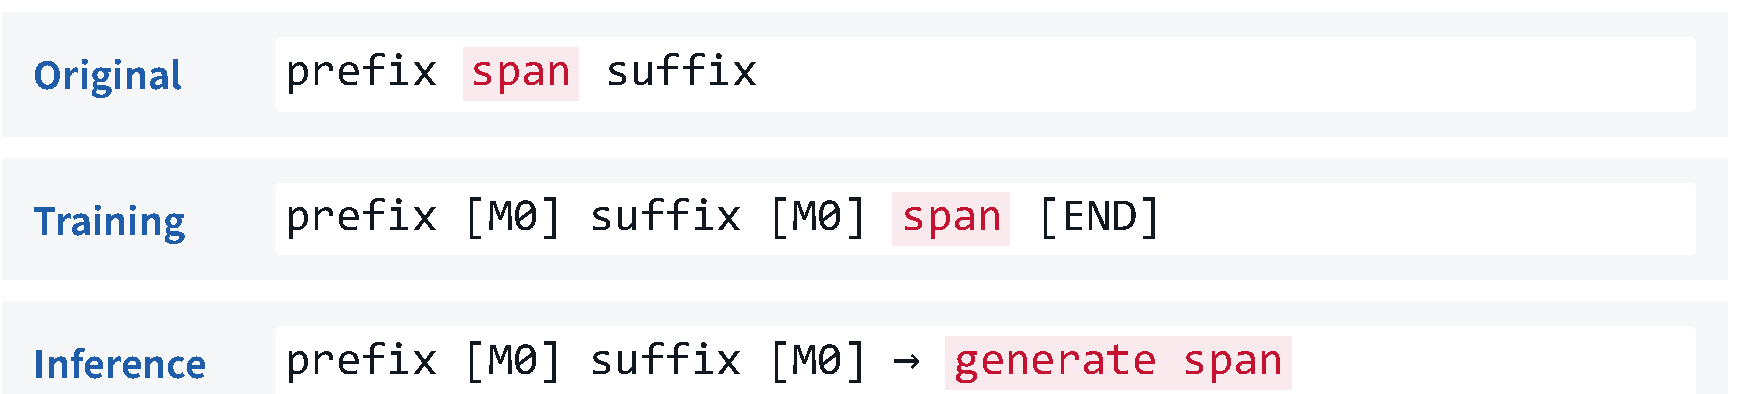
\includegraphics[width=\textwidth]{figures/Infilling重排序与哨兵位置.pdf}
\caption{第一次出现的 M0 标出原位置，第二次出现的 M0 引导生成待插入片段；END 结束片段。图中使用课堂简化记号。来源：官方课件第 15 页；对应口述 00:24:03--00:25:33。}
\end{figure}

这一操作没有要求模型在原程序顺序中看到未来 Token。因果模型仍从左向右读取\emph{重排后的}序列；原程序中处于右侧的代码，被放到了待生成片段之前。

为把该机制写成条件概率，先令输入包含左侧、位置标记、右侧以及生成标记，再逐项生成缺口内容。这是对课件机制的记号展开。
$$
c=[\ell;M_0;r;M_0],\qquad
p_\theta(s\mid c)=\prod_{i=1}^{|s|}p_\theta(s_i\mid c,s_{<i}).
$$
\begin{itemize}
\item $\ell$、$r$：缺口左侧与右侧的 Token 序列。
\item $M_0$：关联同一个缺口位置与待生成片段的哨兵标记。
\item $[\,;\,]$：按所列顺序拼接序列；$c$ 是模型生成时已给定的上下文。
\item $s$：待填充的 Token 序列；$|s|$ 为其长度，$s_i$ 是第 $i$ 项，$s_{<i}$ 是此前生成的项。
\item $p_\theta$：参数为 $\theta$ 的模型条件概率；$\prod$ 将各项概率相乘。
\end{itemize}

多缺口使用不同哨兵关联各位置，依次生成对应片段。课程据此列出代码中间补全、类型推断、生成注释以及变量改名等用途。采样多少缺口、每段多长，会影响模型在训练中见到的编辑任务分布。课堂讨论强调通常较少缺口、偶尔更多缺口的采样方式；具体实现应查看研究中的采样规则，不能把临场口述的估计当作精确参数。

\begin{importantbox}{Infilling 的关键是改变条件信息}
在生成候选时已经看到右侧代码，模型就能主动选择与后续内容兼容的片段。先仅凭左侧生成候选，再使用右侧内容筛选，也能获益，但候选集合中可能始终没有合适答案。
\end{importantbox}

\subsection{实验：右侧信息用于生成，比仅用于重排更有效}
课程给出的 InCoder 实验，从 HumanEval 的参考实现构造单行和多行缺口，填回候选后运行函数测试。三行结果分别对应：只凭左侧生成一项；只凭左侧生成十项，再用完整上下文重排；直接用双侧上下文生成。

\begin{figure}[H]
\centering
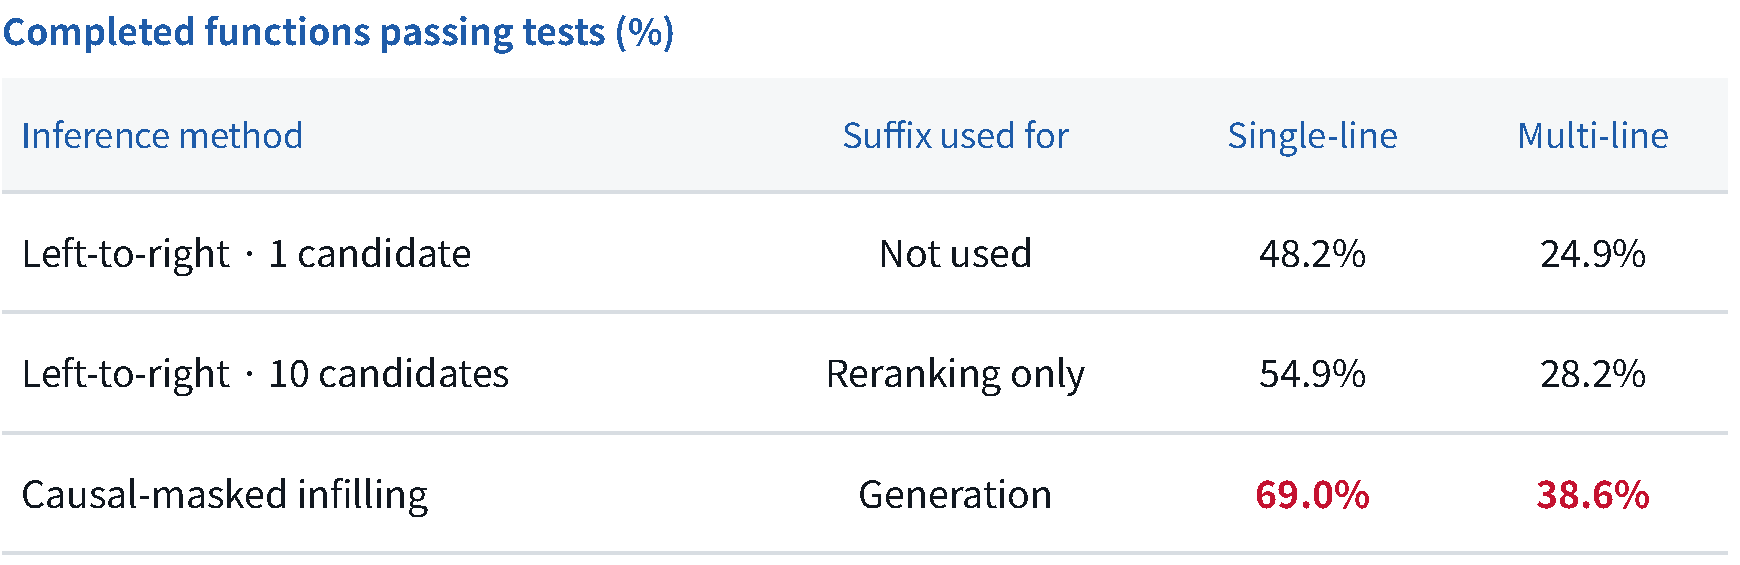
\includegraphics[width=\textwidth]{figures/InCoder右侧上下文补全实验.pdf}
\caption{单行与多行 Infilling 的完成函数测试通过率，保留了三种推断方式对右侧信息的不同用法。来源：官方课件第 16 页；对应口述 00:25:33--00:26:22。}
\end{figure}

单行通过率从 48.2\% 提高到 54.9\%，再提高到 69.0\%；多行从 24.9\% 提高到 28.2\%，再提高到 38.6\%。这些是该研究中派生补全任务的结果，不能直接作为完整仓库修复成功率。

第二个问题是：增加中间补全能力，会不会削弱普通从左向右的生成？课件展示相同 52B Token 训练预算下的目标消融。原论文中对应比较使用 1.3B 参数模型：因果掩码目标的 HumanEval / MBPP pass@1 为 8.0\% / 10.9\%，普通语言模型目标为 6.0\% / 8.9\%。

\begin{figure}[H]
\centering
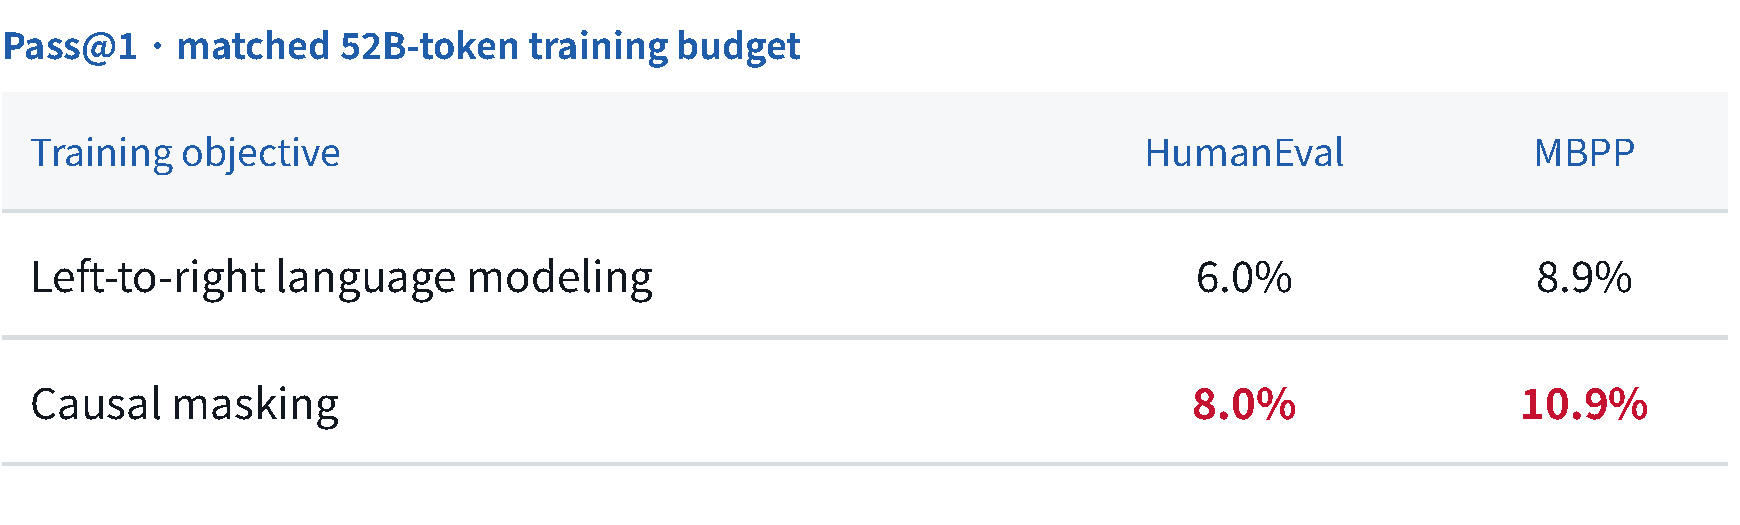
\includegraphics[width=\textwidth]{figures/InCoder训练目标消融.pdf}
\caption{相同训练预算下，Infilling 目标保留了普通代码生成能力；数字属于该研究的 1.3B 模型消融。来源：官方课件第 17 页；对应口述 00:26:22--00:28:08。}
\end{figure}

\begin{warningbox}{实验支持的结论需要保留条件}
这些结果支持在该训练设置下兼顾中间补全与普通生成。它们没有证明所有模型、所有数据混合与所有 Infilling 比例都完全没有代价。比较时应区分推断方式实验和训练目标消融，后者的模型规模也不同。
\end{warningbox}

\subsection{从开发记录中构造更多训练任务}
Infilling 把静态源码转成编辑任务。开发过程还有更多材料，可以帮助模型学习怎样修改与检查程序。课件归纳了四类信号。

\begin{center}
\small
\begin{tabularx}{\textwidth}{L{2.4cm}XX}
\toprule
材料 & 构造的任务 & 学习方向 \\
\midrule
Commit diff & 修改前代码与提交说明 $\rightarrow$ 修改后代码或 diff & 理解修改意图，形成编辑 \\
错误诊断 & 出错代码与错误信息 $\rightarrow$ 修复 & 从报错定位原因并改正 \\
测试结果 & 程序与测试通过情况 $\rightarrow$ 奖励 & 强化满足已检查行为的输出 \\
执行轨迹 & 程序 $\rightarrow$ 执行行与状态 & 学习程序运行时怎样变化 \\
\bottomrule
\end{tabularx}
\end{center}

诊断数据不必全部人工创造。讲者特别指出，公开 CI 历史包含一个版本失败、后续修改通过并最终合并的记录，可以提供代码、错误与修复之间的关联。Stack Overflow、issues 和 pull requests 也能提供相关信息。若由 Agent 实际执行任务，还可以收集搜索、修改、测试与反馈的轨迹。

执行轨迹又提供另一种监督：通过程序插桩和运行，记录执行到哪一行、变量状态或某处输出，再训练模型预测这些变化。课程把这个方向与后面的代码行为预测联系起来。这里要区分“预测运行结果”与“实际执行程序”：预测可以成为训练信号或建模任务，真实执行才提供所使用环境中的观察结果。

这些信号的质量都依赖输入、结果与修改之间的正确关联。例如，一个 CI 失败后来消失，仍要检查究竟是修复了错误、修改了测试，还是外部环境发生变化。将开发记录转换成训练任务，需要保留任务边界和环境条件。

\subsection{本章小结}
定向适配通过数据混合与相关文件组织，加强代码专长和跨文件能力。Infilling 把两侧上下文移到生成位置之前，使自回归模型能够编辑已有程序；课堂实验同时检查了补全收益和普通生成能力。提交、报错、测试与执行轨迹把训练信号进一步扩展到开发过程。下一步需要回答：怎样评价候选程序，怎样把评价结果变成可靠反馈？

\subsection{拓展阅读}
\begin{itemize}
\item \href{https://arxiv.org/abs/2204.05999}{InCoder}：重排序、双侧上下文和中间补全实验。
\item \href{https://arxiv.org/abs/2409.12186}{Qwen2.5-Coder Technical Report}：数据混合与仓库级上下文训练；\href{https://arxiv.org/abs/2308.12950}{Code Llama}：从基础模型到代码专长的训练路线。
\end{itemize}

\clearpage
\begingroup
\setlength{\parskip}{.2em}
\section{单步代码生成：以行为为中心的评测}

模型生成一段代码之后，评价者需要判断它是否完成了要求。这里有两个可以观察的对象：代码的表示，以及代码运行后的行为。前者便于与参考答案比较，后者更接近程序实际承担的功能。课程先介绍表示层面的指标，再说明执行测试为何成为代码生成的重要反馈来源。

\subsection{参考答案相似度能说明什么}

最直接的指标是精确匹配：生成代码是否与人工参考代码完全一致。BLEU-4 则允许部分匹配，比较 Token 的 1 到 4 元组重叠，并对过短候选施加惩罚。这类方法不需要准备完整运行环境，但程序中一个很小的文本差别就可能改变行为。

假设输入 \texttt{x} 被明确规定为整数，要求判断它是否为正数。三种表达式的关系如下：

\begin{center}
\begin{tabularx}{\textwidth}{L{3.1cm}L{5.2cm}X}
\toprule
表达式 & 与参考表达式的关系 & 实际行为 \\
\midrule
\texttt{return x > 0} & 参考实现 & 零返回假，正数返回真 \\
\texttt{return x >= 0} & 仅改变一个运算符 & 零返回真，违反要求 \\
\texttt{return not (x <= 0)} & 表面写法变化较大 & 在整数输入范围内等价 \\
\bottomrule
\end{tabularx}
\end{center}

因此，相似度指标可能给错误程序很高的分数，也可能降低另一种正确实现的分数。限定整数输入也有实际意义：等价性判断需要依据任务规定的输入域，不能把例子中的结论自动推广到所有对象和特殊数值。

CodeBLEU 在词法匹配之外加入代码结构的信息。抽象语法树（AST）描述表达式、语句与分支的组织方式；数据流描述变量值从何处产生、又被哪些操作使用。它把这些信号组合起来，降低只看表面 Token 的局限。

\begin{figure}[H]
\centering
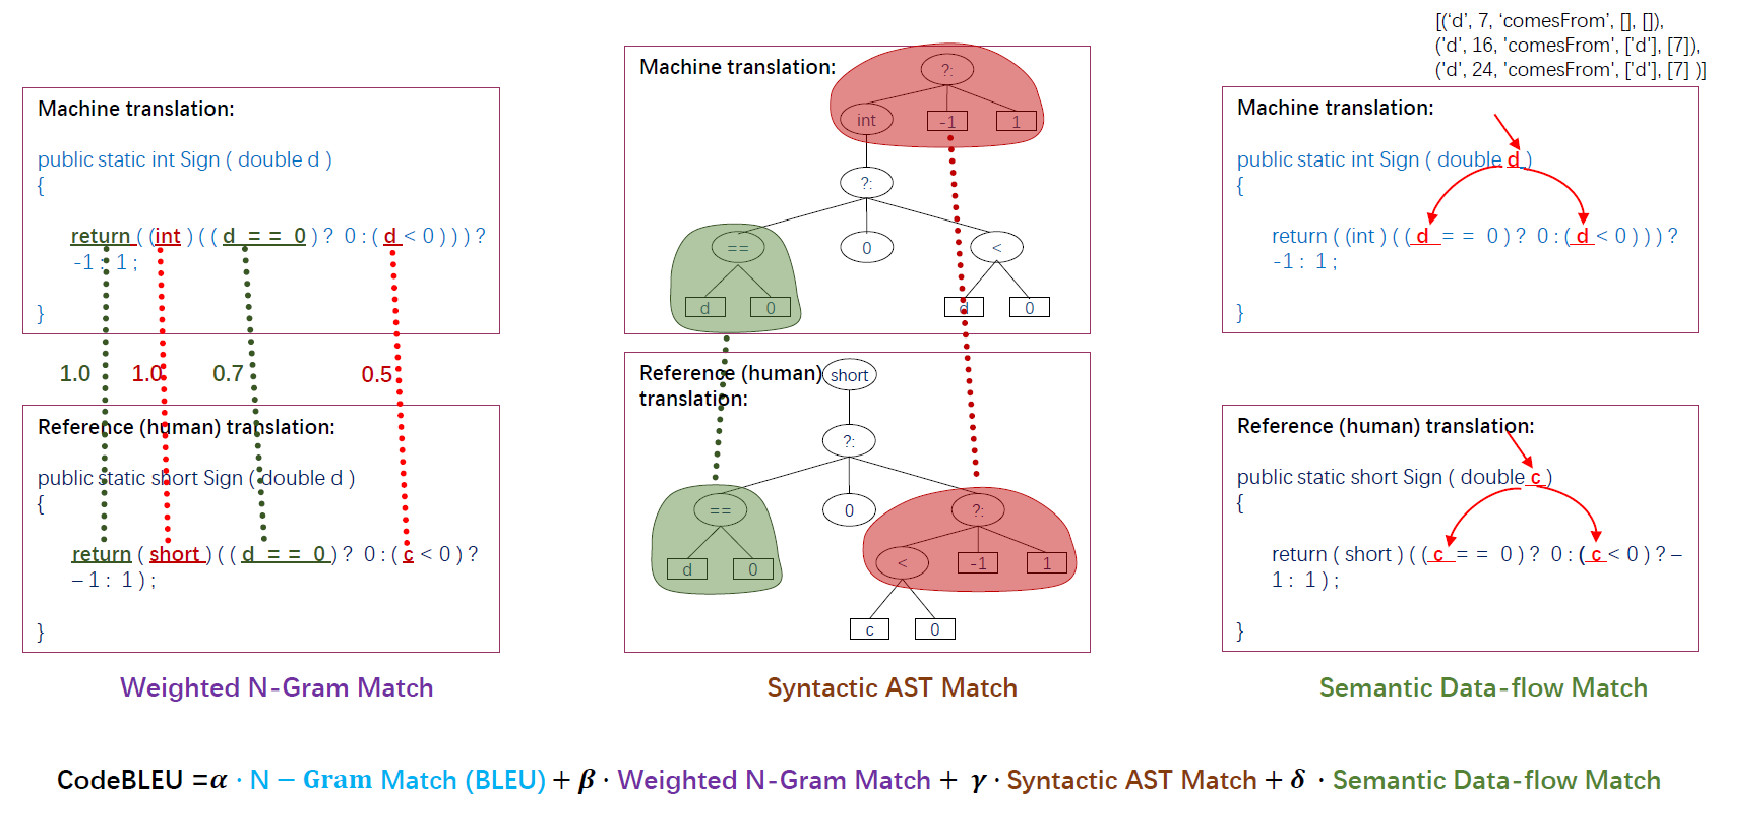
\includegraphics[width=\textwidth]{figures/CodeBLEU的词法语法与数据流比较.pdf}
\caption{CodeBLEU 对照加权词法、AST 与数据流信息；图中的绿色与红色区域标示不同匹配情况。来源：官方课件第 21 页；对应口述 00:32:17--00:33:13。}
\end{figure}

课件中的加权组合可以写成下面的形式。它表达的是多个相似度信号共同参与评分，而没有声称这些信号能完整证明功能等价。
$$
\mathrm{CodeBLEU}=\alpha B+\beta B_{\mathrm{w}}+\gamma A+\delta D.
$$
\begin{itemize}\setlength{\itemsep}{2pt}\setlength{\parsep}{0pt}\setlength{\topsep}{4pt}
\item $\mathrm{CodeBLEU}$：组合后的代码相似度分数。
\item $B$：普通 Token 元组匹配分数，即 BLEU 部分。
\item $B_{\mathrm{w}}$：加权 Token 元组匹配分数，对不同代码 Token 赋予不同重要性。
\item $A$：AST 结构匹配分数。
\item $D$：数据流匹配分数。
\item $\alpha,\beta,\gamma,\delta$：各部分的权重，通常按归一化权重设置；具体取值属于评测配置。
\end{itemize}

另一条路线是比较学习得到的表示。CodeBERTScore 将提示和各自的代码片段输入代码编码器，为代码 Token 得到上下文向量。对于一个片段中的 Token，寻找另一个片段中最相似的 Token；再从候选覆盖参考、参考覆盖候选两个方向汇总，得到类似精确率、召回率及 F 分数的结果。这里的匹配允许多个 Token 选择同一个对应项，并不要求严格的一一配对。

\begin{figure}[H]
\centering
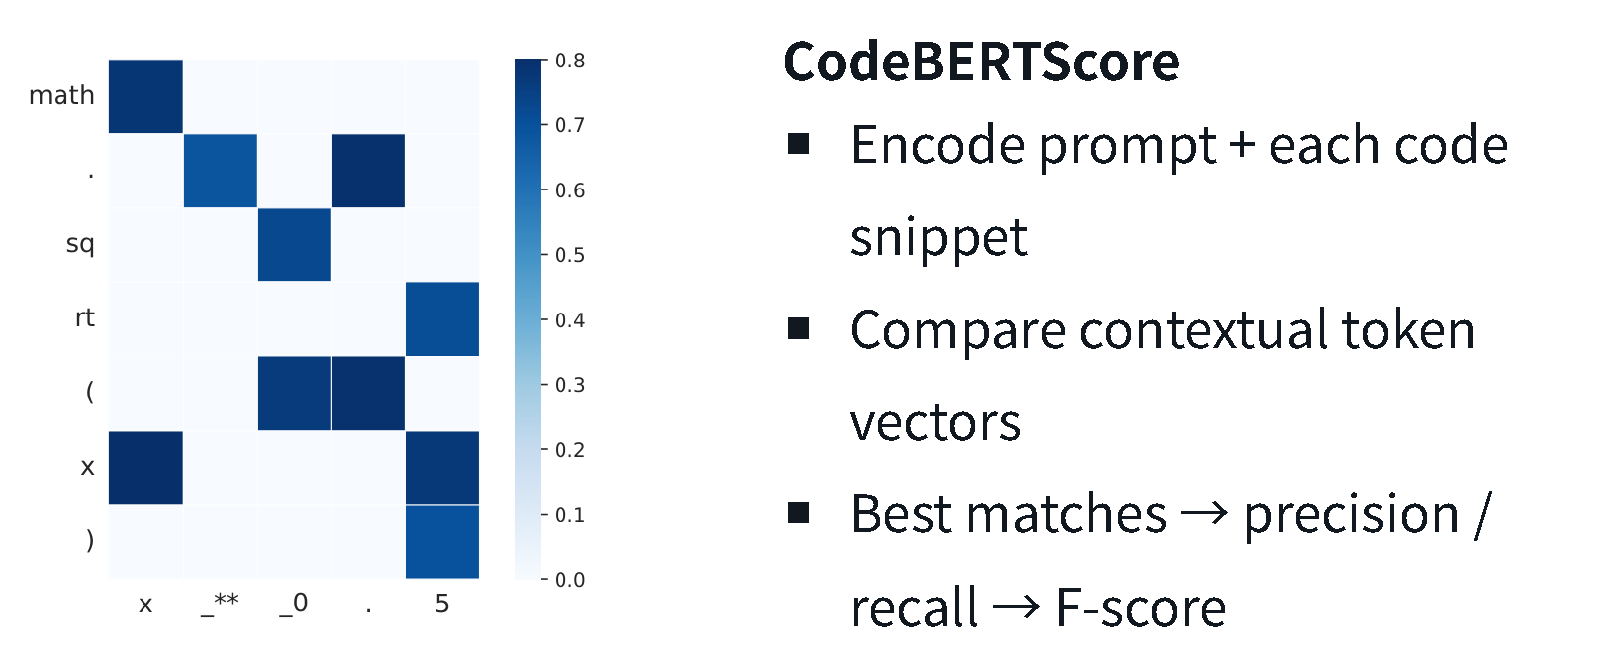
\includegraphics[width=.96\textwidth]{figures/CodeBERTScore的上下文Token相似度.pdf}
\caption{上下文向量的相似度矩阵支持不同写法之间的软匹配；深色格子表示较高的 Token 相似度。来源：官方课件第 22 页；对应口述 00:33:13--00:34:04。}
\end{figure}

\begin{importantbox}{表示层面的评分仍然是代理信号}
精确匹配、BLEU、CodeBLEU 和 CodeBERTScore 分别使用文本、结构或学习得到的表示。它们可以衡量与参考实现的接近程度，但高分本身不能证明所有输入上的行为正确。
\end{importantbox}

\subsection{执行检查：接受不同的正确实现}

执行评测提供一组输入与预期结果，在准备好的环境中运行候选程序，再比较结果。对于“整数是否为正”这个例子，输入 $-1$、$0$、$1$ 就能揭示 \texttt{x >= 0} 在边界处的错误。无论候选采用哪种语法，只要满足这些检查，都可以通过这一组测试。

\begin{figure}[H]
\centering
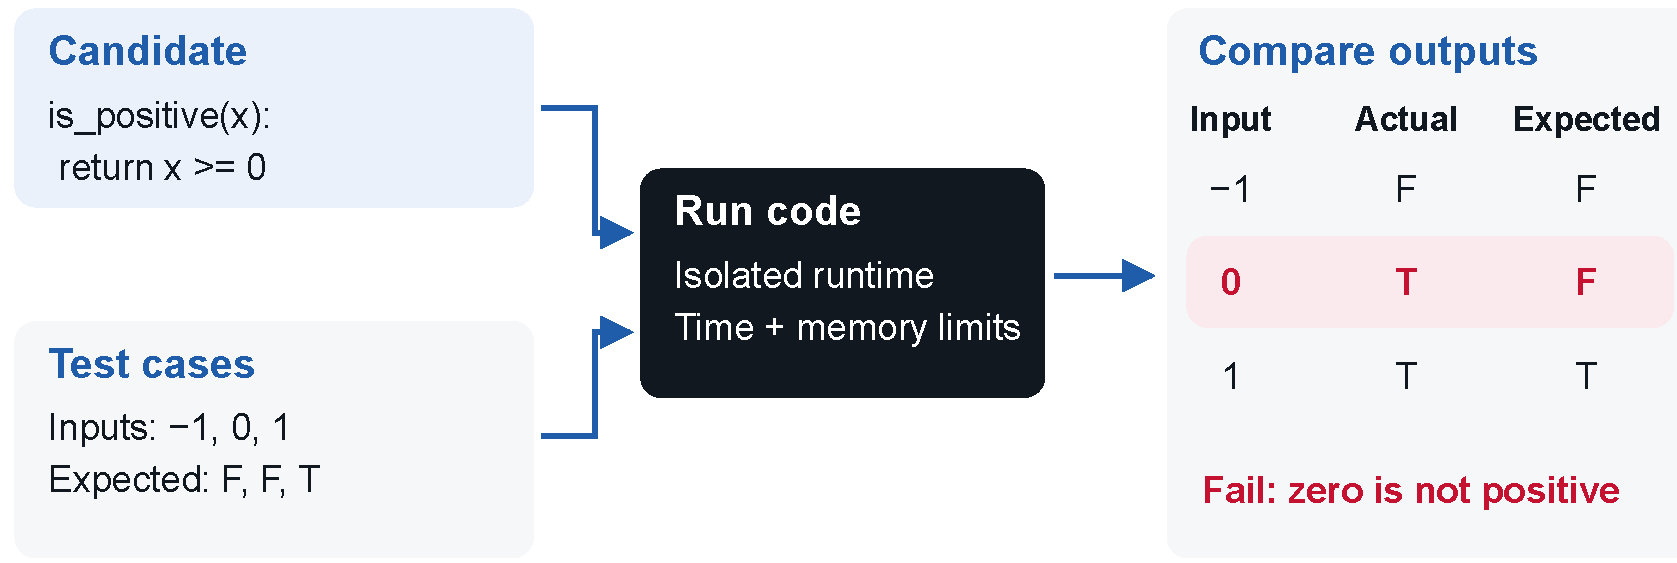
\includegraphics[width=\textwidth]{figures/执行测试发现零值边界错误.pdf}
\caption{测试将候选代码转化为可观察的行为：零值用例直接区分 \texttt{>} 与 \texttt{>=}。来源：官方课件第 23 页；对应口述 00:34:04--00:34:42。}
\end{figure}

这种评价方式绕开了“必须与参考代码长得相同”的要求，也能通过执行发现语义错误。不过，测试集合是有限的。它既可能漏掉错误，也可能加入输入说明中没有交代的条件。

\begin{warningbox}{两类测试偏差会直接影响模型分数}
\textbf{错误实现通过}：测试没有覆盖关键边界或组合，导致程序在测试之外仍然出错。\textbf{合理实现被判失败}：任务说明缺少某项要求，测试却要求实现它。讲者举例：要求界面右上角出现“Learn more”按钮，却额外检查未说明的背景色。这两类问题都需要同时核对规格与测试。
\end{warningbox}

运行环境也是评分机制的一部分。仅依赖 Python 标准库的函数比较容易部署；真实仓库还要安装依赖、固定兼容版本、准备构建工具，并限制候选程序的运行时间、内存与可访问资源。容器常被用来封装依赖，但隔离是否充分仍取决于具体配置。依赖版本漂移导致的测试失败，不能自动解释为模型能力下降。大型仓库的测试成本还会限制能评估多少候选和多少任务。

\subsection{从函数补全到竞赛程序}

课程用 HumanEval 和 CodeContests 说明单步任务的范围。HumanEval 包含 164 个手工编写的 Python 函数任务，模型根据函数签名与文档字符串生成实现，再由隐藏单元测试检查。它主要测试从文字规格到独立函数的能力，不能完整代表维护大型软件仓库的工作。前文实验中的 MBPP 也是常用的 Python 程序生成基准，用自然语言任务与测试考察相对基础的编程能力。

CodeContests 则包含 Codeforces 等来源的竞赛题，输入是题目陈述，输出通常是完整程序，需要编译或解释执行，并满足输入输出格式及资源限制。对困难题目，要求一次生成就全部正确，本身就是很强的要求。

\subsection{pass@k：多个尝试中至少有一个通过}

pass@1 检查一次采样的程序是否通过所有测试；pass@k 关注 $k$ 次采样中是否至少有一个通过。这有助于区分“一次就答对”和“能够在多个候选中产生正确答案”。

为说明概率关系，先作一个\textbf{教学简化}：某道题每次独立采样的通过概率相同。于是，至少一次通过的概率等于一减去全部失败的概率。
$$
\mathrm{pass@}k=1-(1-p)^k.
$$
\begin{itemize}\setlength{\itemsep}{2pt}\setlength{\parsep}{0pt}\setlength{\topsep}{4pt}
\item $\mathrm{pass@}k$：该任务在 $k$ 次采样中至少产生一个通过程序的概率。
\item $p$：在固定模型、提示和采样设置下，单次采样通过全部测试的真实概率。
\item $k$：允许采样的候选数，取正整数。
\end{itemize}

评测者通常不知道真实的 $p$。HumanEval 原始论文通过生成更多样本，再统计正确样本数，估计指定预算下的 pass@k。下面是论文估计式的\textbf{教学展开}：从已生成的样本池中不放回取出 $k$ 个，全部落在错误样本中的组合占比，就是一次都没有通过的比例。
$$
\widehat{\mathrm{pass@}k}
=1-\frac{\binom{n-c}{k}}{\binom{n}{k}},\qquad n\ge k.
$$
\begin{itemize}\setlength{\itemsep}{2pt}\setlength{\parsep}{0pt}\setlength{\topsep}{4pt}
\item $\widehat{\mathrm{pass@}k}$：一项任务的 pass@k 估计值；整个基准还需要对各任务求平均。
\item $n$：为该任务生成的总样本数。
\item $c$：这 $n$ 个样本中通过所有测试的样本数，满足 $0\le c\le n$。
\item $k$：所要报告的候选预算，满足 $1\le k\le n$。
\item $\binom{a}{k}$：从 $a$ 个对象中选择 $k$ 个的组合数；当 $a<k$ 时取零。
\end{itemize}

例如，10 个候选中有 2 个通过，预算为 3 时，估计值为 $1-56/120\approx0.533$。在独立同分布采样假设下，这一统计量是原论文使用的无偏估计。直接把经验通过率 $c/n$ 代入上一条概率式，一般会得到有偏估计。对于会根据前一次失败结果继续修改的 Agent 轨迹，也不能直接把这个独立采样解释照搬过来。

\begin{figure}[H]
\centering
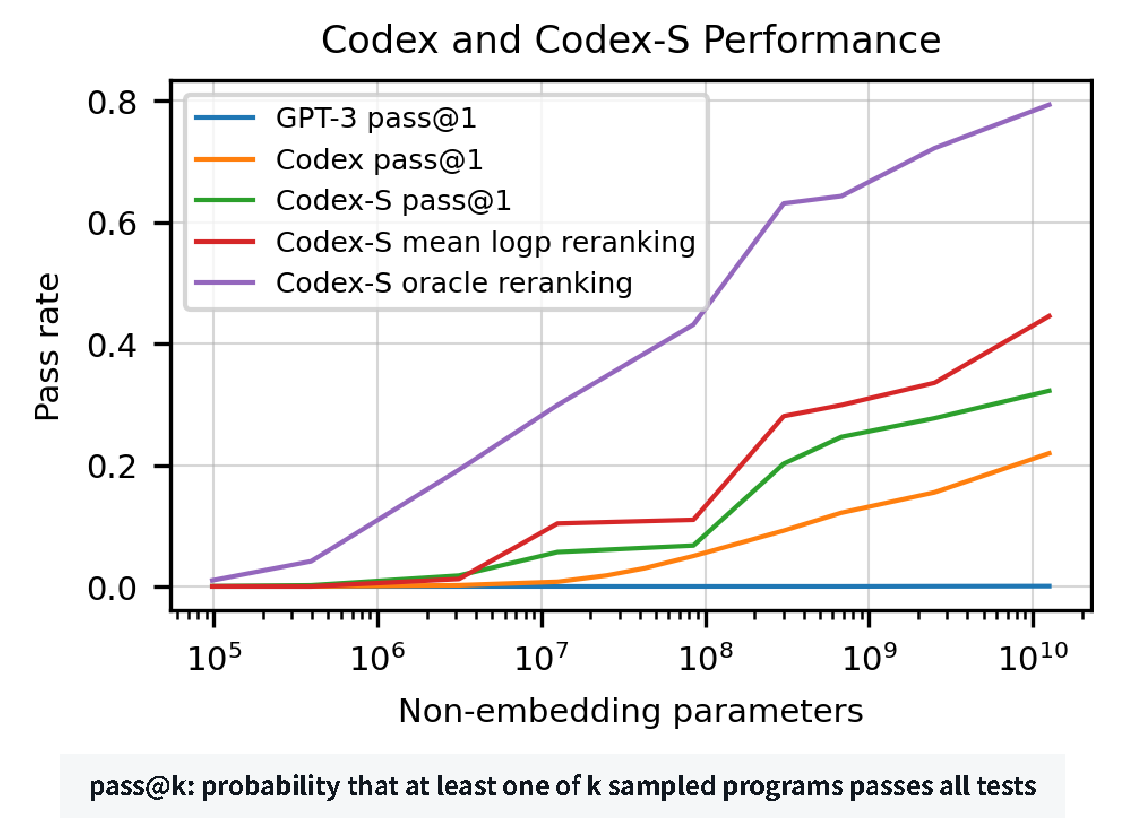
\includegraphics[width=.84\textwidth]{figures/历史Codex规模采样与选择策略.pdf}
\caption{2021 年 HumanEval 研究中的模型规模与选择方式。图中 Codex 指当年的代码模型；mean logp 与 oracle 曲线从 100 个采样候选中选择一个，不能与 pass@1 按同一候选预算解释。来源：官方课件第 26 页；对应口述 00:39:30--00:40:46。}
\end{figure}

\begin{warningbox}{生成到正确候选，和选出正确候选，是两个能力}
pass@k 只要求样本集合中存在一个通过程序。实际使用还需要找出它：可以运行可用测试，或使用评分器排序。图中的 oracle 能根据正确性挑选候选，属于理想选择条件；按平均 Token 对数概率选择则仍可能选错。比较结果时，要一起报告候选数、采样设置、选择器以及执行预算。
\end{warningbox}

\subsection{功能通过之后，还有非功能要求}

“输出正确”没有覆盖软件的全部要求。相同功能还可能要求更快、少用内存、更易维护或避免安全缺陷。课堂问答据此引出 NoFunEval：对已有程序提出非功能修改要求，再检查改进。课件中的 397 项代码编辑任务采用不同验证方式，不能用一个功能测试分数替代全部目标。

\begin{figure}[H]
\centering
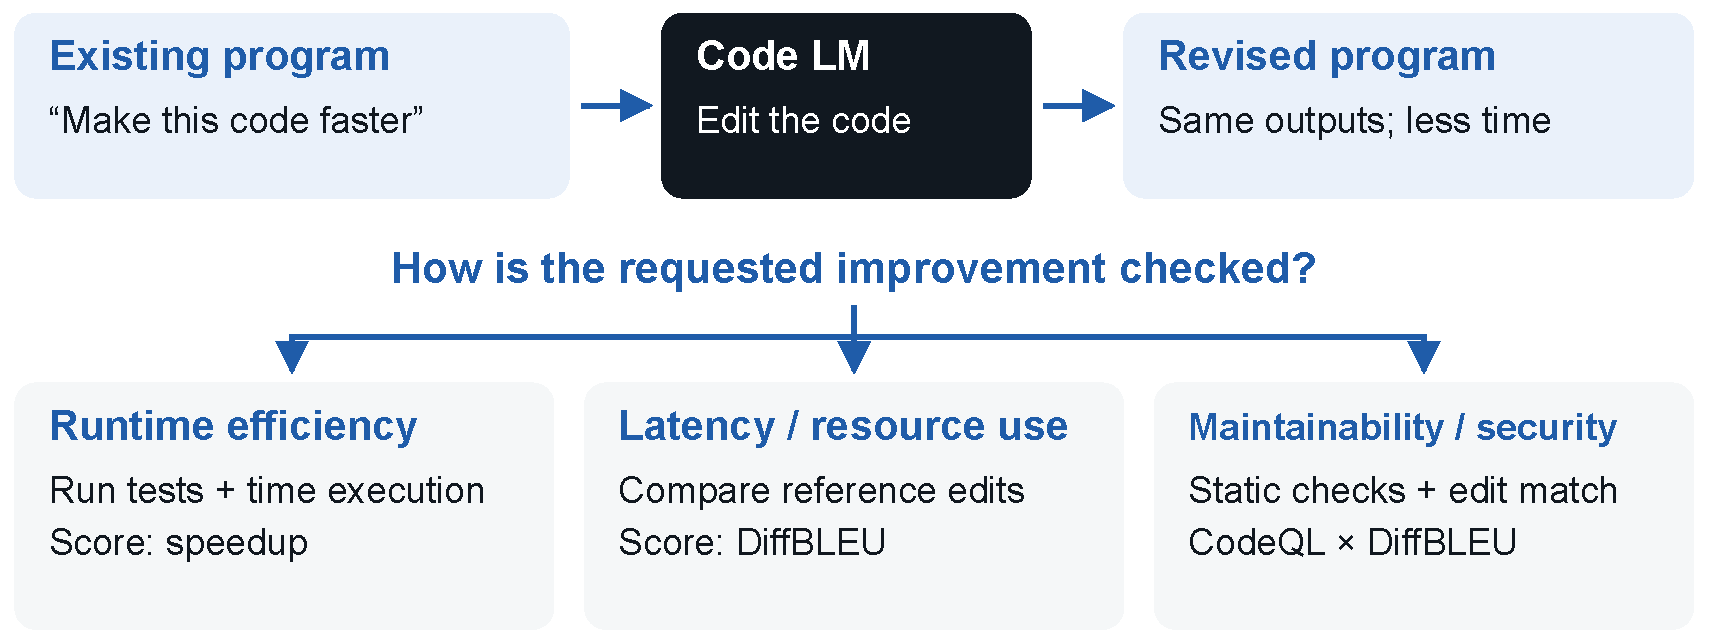
\includegraphics[width=\textwidth]{figures/非功能要求的不同验证方式.pdf}
\caption{非功能目标需要选择相应的验证信号：直接测量运行效率、比较参考修改，或结合静态检查。来源：官方课件第 27 页；对应口述 00:40:46--00:42:15。}
\end{figure}

运行效率可以先检查功能保持，再测量执行时间并计算加速比。NoFunEval 的延迟和资源使用任务因目标平台各异，以 DiffBLEU 衡量修改与参考修改的接近程度；可维护性和安全任务结合 CodeQL 静态检查与修改匹配。这里，DiffBLEU 是编辑相似度代理，不等于已经在所有目标平台上测得更低延迟；没有某项静态告警，也不意味着代码的所有安全属性都已得到证明。

\subsection{本章小结}
\begin{itemize}\setlength{\itemsep}{2pt}\setlength{\parsep}{0pt}\setlength{\topsep}{4pt}
\item 表示相似度提供方便的代理信号；执行检查允许不同的正确实现，但结论受测试规格和环境约束。
\item HumanEval、MBPP 与竞赛程序覆盖不同任务范围。分数必须与题目类型及评测设置一起理解。
\item pass@k 衡量多次采样中至少一次通过，实际选择候选还需要另一个可靠机制。
\item 功能、运行效率、资源使用及代码质量需要各自适合的检查方式。
\end{itemize}

\subsection{拓展阅读}
\begin{itemize}\setlength{\itemsep}{2pt}\setlength{\parsep}{0pt}\setlength{\topsep}{4pt}
\item \href{https://arxiv.org/abs/2107.03374}{Chen 等：HumanEval、功能正确性评价与 pass@k 估计}。
\item \href{https://arxiv.org/abs/2401.15963}{Singhal 等：NoFunEval 的非功能任务与指标}。
\end{itemize}

\endgroup
\clearpage
\begingroup
\setlength{\parskip}{.2em}
\section{从测试反馈到可交互的代码修复}

可执行测试不仅能评价模型，还能成为训练反馈。由此可以训练模型更常生成能通过的程序。接着，课程把工作环境从一个独立题目扩展到已有仓库：模型需要找到相关实现，修改文件，并利用运行结果决定后续行动。

\subsection{用测试奖励训练单步代码模型}

单步代码任务的强化学习流程比较直接：针对题目采样“推理过程加最终代码”，运行最终代码的测试，将通过或失败转成奖励，再更新模型。下一轮用更新后的模型继续采样。训练时经历许多轮更新，仍然可以把每个题目的作答视作一次生成；这与部署时让 Agent 连续调用工具是两种不同的循环。

\begin{figure}[H]
\centering
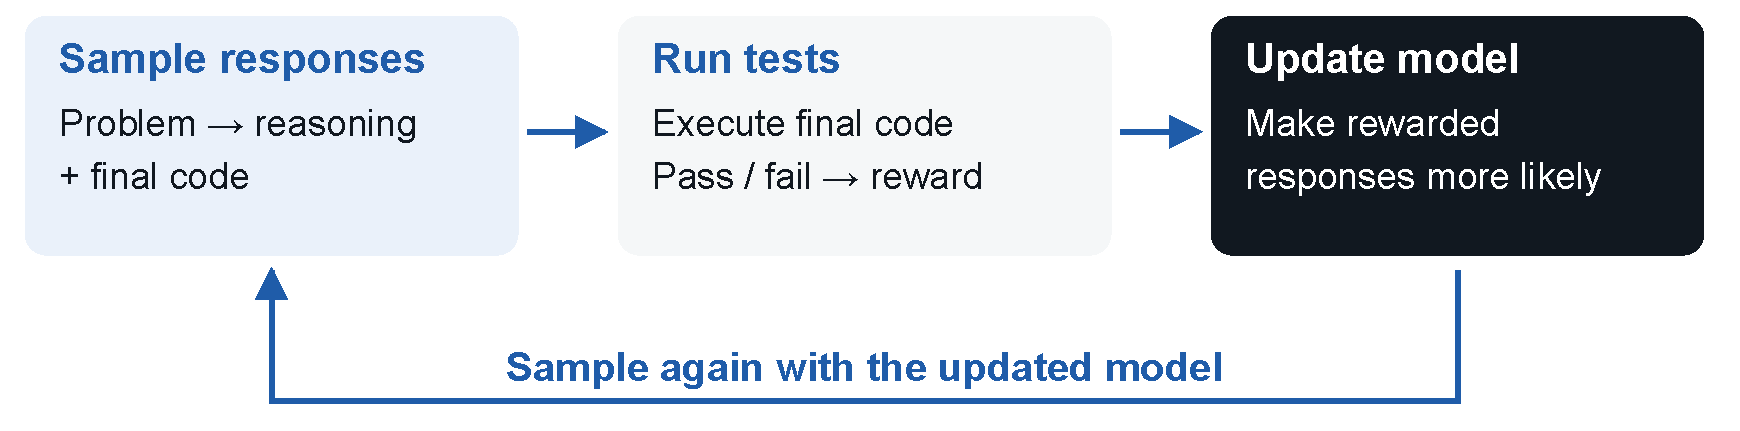
\includegraphics[width=\textwidth]{figures/从测试奖励到模型更新.pdf}
\caption{测试结果进入训练循环：采样响应、执行代码、形成奖励、更新模型。来源：官方课件第 28 页；对应口述 00:42:15--00:44:11。}
\end{figure}

下面用一个\textbf{教学抽象}表示这一目标：提高从题目分布采样后，模型响应获得的平均奖励。实际强化学习方法还需要定义更新规则、稳定化约束与采样设置；课堂没有在此展开具体优化算法。
$$
\max_{\theta}\;
\mathbb{E}_{x\sim\mathcal{D},\,y\sim\pi_{\theta}(\cdot\mid x)}
[R(x,y)].
$$
\begin{itemize}\setlength{\itemsep}{2pt}\setlength{\parsep}{0pt}\setlength{\topsep}{4pt}
\item $\theta$：待更新的模型参数。
\item $\mathcal{D}$：训练题目的分布。
\item $x$：一道训练题目及提供给模型的条件。
\item $\pi_{\theta}(\cdot\mid x)$：在题目 $x$ 下生成响应的模型分布。
\item $y$：采样到的响应，可包含推理文本与最终代码。
\item $R(x,y)$：依据题目和响应得到的奖励；简单情形为最终代码全部通过取 1，否则取 0。
\item $\mathbb{E}$：对题目和响应采样取期望。
\end{itemize}

这种反馈无需逐条人工标注推理步骤，也能鼓励有助于解题的推理。但结果奖励来自测试，测试的盲区和未说明的要求也会进入训练目标。长推理文本是否有用，应根据最终程序及其检查结果判断，不能仅凭长度下结论。

\subsection{推理如何同时处理正确性与效率}

课件用求 $1+\cdots+n$，且 $0\le n\le10^{12}$ 的例子说明推理的作用。直接逐个累加，在小输入上能产生正确结果，但极大输入下需要执行过多步骤。将首尾配对，可以得到一个执行步骤数不随 $n$ 线性增长的表达式。
$$
\sum_{i=1}^{n}i=\frac{n(n+1)}{2}.
$$
\begin{itemize}\setlength{\itemsep}{2pt}\setlength{\parsep}{0pt}\setlength{\topsep}{4pt}
\item $n$：非负整数上界；本例最大取 $10^{12}$。
\item $i$：求和中的整数索引。
\item $\sum_{i=1}^{n}$：从 1 加到 $n$；$n=0$ 时为空和，取 0。
\end{itemize}

下面是对课件三条思路的教学改写，用 Python 的任意精度整数保存结果。高效版本的算术操作数是常数；若分析位复杂度，整数乘法的成本仍会随数值位数变化。

\par\noindent\begin{minipage}{\textwidth}
\begin{lstlisting}[caption={教学改写：逐项累加、配对公式与误写公式}]
def iterative_sum(n):
    return sum(range(n + 1))

def paired_sum(n):
    return n * (n + 1) // 2

def mistranscribed_sum(n):
    return n * (n - 1) // 2
\end{lstlisting}
\end{minipage}

第三种写法表面上很像公式，却在 $n=1$ 时已经返回 0。推导后检查 0 和 1 等边界，能排除这种低成本错误。竞赛题通常还设有时间限制，因此即使奖励只表述为通过或失败，超时也会间接约束程序效率；不过，时间上限以内的两个正确程序仍可能得到相同奖励。

\subsection{DeepCoder：训练预算与评估预算分开理解}

课件展示 DeepCoder 的 LiveCodeBench 训练曲线。训练中允许的响应 Token 预算从 16K 提高到 32K，曲线呈现总体提升与局部波动。最后的星标使用 64K 评估预算；它来自最佳检查点的推理时扩展，没有再进行一阶段 64K 强化学习。图中的 K 表示 1,000 个 Token，所扩展的是模型响应的生成预算。

\begin{figure}[H]
\centering
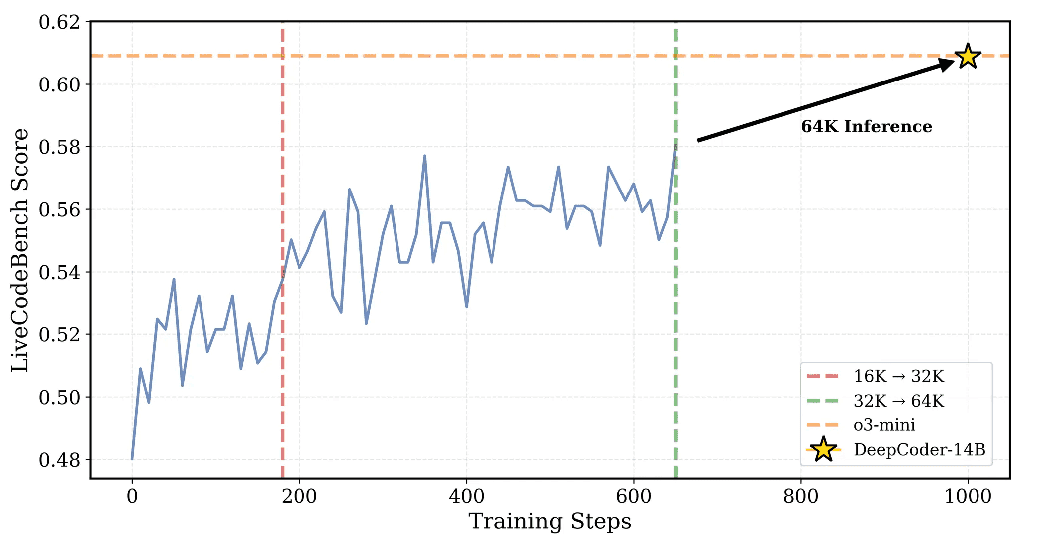
\includegraphics[width=.90\textwidth]{figures/DeepCoder训练与评估预算的变化.pdf}
\caption{DeepCoder 的训练和推理时扩展。绿色标记后的 64K 终点属于评估时增加响应预算；橙色虚线为该历史实验中的 o3-mini 对照。来源：官方课件第 30 页；对应口述 00:42:15--00:44:11。}
\end{figure}

这个实验同时涉及训练反馈和推理预算，因而不能把所有提升都归结为“单纯多训练几步”，也不能把历史曲线作为当前模型排名。它支持的教学结论是：可验证的代码结果能用于强化学习；对需要复杂推理的任务，作答时允许的计算量同样影响结果。

课堂还讨论代码注释与可读性。讲者提出，训练代码中已有注释，或生成注释可能为后续推理提供空间，都是注释出现的可能原因；这些是解释性假设，没有给出特定闭源模型的训练证据。对于可读性，可以收集人的质量判断，训练相应奖励模型，再在后训练中纳入该信号。测试通过率与可读性反馈承担的目标不同，通常需要分别考虑。

\subsection{仓库级任务：定位、编辑、验证}

单步题目已经把相关信息放进提示，要求一次输出程序。仓库级问题则从 Issue 和现有文件开始：相关实现可能不在当前上下文里，修改可能影响其他调用者，执行结果会暴露第一次推断的不足。课程将这一过程分成三个动作：
\begin{enumerate}\setlength{\itemsep}{2pt}\setlength{\parsep}{0pt}\setlength{\topsep}{4pt}
\item \textbf{定位（localize）}：找到应当修改的位置，并重现问题。
\item \textbf{编辑（edit）}：改变实现，使它符合要求。
\item \textbf{验证（verify）}：运行针对问题的检查及相关回归检查，必要时返回前面的步骤。
\end{enumerate}

\begin{figure}[H]
\centering
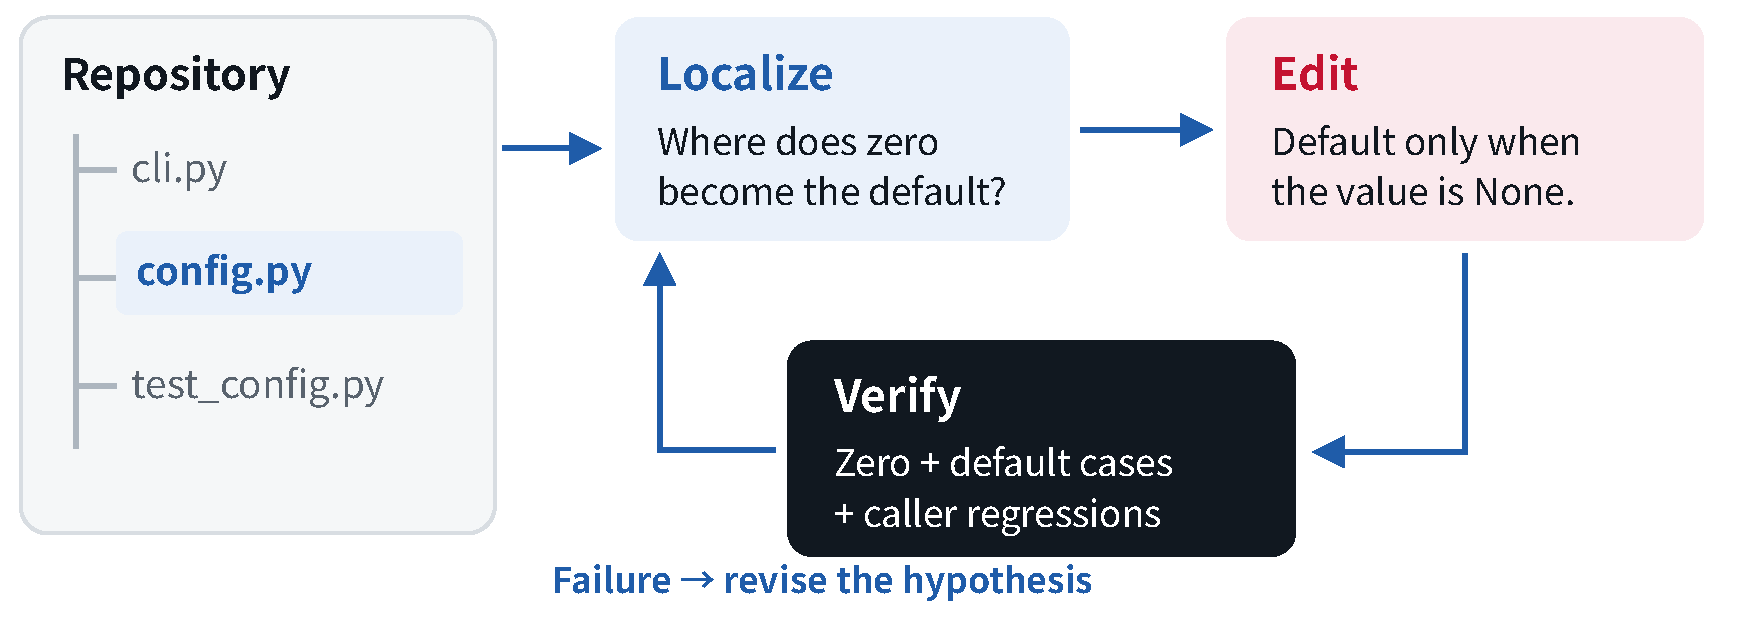
\includegraphics[width=\textwidth]{figures/定位编辑验证的反馈循环.pdf}
\caption{仓库状态、修复假设与执行反馈构成循环；验证失败时需要重新检查原因或修改。来源：官方课件第 33 页；对应口述 00:47:16--00:49:45。}
\end{figure}

运行例子是配置中的重试次数。预期行为为：缺少 \texttt{retries} 或明确设置为 \texttt{None} 时用默认值 3，设置为 0 时保留 0。定位时可以搜索 \texttt{retries}，检查配置加载与使用路径。原实现使用 \texttt{or 3}，会把 0 等假值也换成默认值；重现零值测试即可得到“实际 3，预期 0”的失败。

以下补全为函数的代码保留了课件的修复语义。修改范围集中在默认规则，零值仍保留，缺失键则由 \texttt{get} 返回 \texttt{None} 后使用默认值。

\par\noindent\begin{minipage}{\textwidth}
\begin{lstlisting}[caption={课件默认规则的教学补全：明确区分 None 与假值}]
def buggy_retry_count(config):
    return config.get("retries") or 3

def retry_count(config):
    value = config.get("retries")
    return 3 if value is None else value
\end{lstlisting}
\end{minipage}

验证同时覆盖问题用例与原来应当保留的默认行为。下面的测试与课件四种情形一致；在真实仓库中，还需要运行与调用者及修改范围有关的现有测试。

\par\noindent\begin{minipage}{\textwidth}
\begin{lstlisting}[caption={教学补全：零值、缺失值、None 和正数的四个回归用例}]
import unittest

class RetryTests(unittest.TestCase):
    def test_config_values(self):
        cases = [
            ({}, 3),
            ({"retries": None}, 3),
            ({"retries": 0}, 0),
            ({"retries": 2}, 2),
        ]
        for config, expected in cases:
            with self.subTest(config=config):
                self.assertEqual(retry_count(config), expected)
\end{lstlisting}
\end{minipage}

若把测试中的调用换成 \texttt{buggy\_retry\_count}，零值子用例失败；调用修复后的函数则四种情形都通过。若零值仍变成 3，应继续追踪值在何处变化；若默认用例出现回归，则需重新检查条件。验证输出因此提供下一步行动依据。

\begin{importantbox}{修复闭环依靠可观察的状态变化}
定位提出并检查原因，编辑落实改变，验证检验请求的行为及已有行为。Agent 的价值来自根据新的文件和执行结果继续行动；仅生成一段看似合理的补丁，还没有完成这个闭环。
\end{importantbox}

\subsection{Agentless：把修复组织成固定工作流}

仓库级代码修复也可以用预先安排的工作流完成。Agentless 先从目录结构与 Issue 预测需要修改的文件，再缩小到类、函数和具体行，随后生成候选补丁，并通过复现测试、过滤与排序选出补丁。模型调用与执行仍然存在，但主要阶段由固定流程组织，模型没有在一个通用交互循环中自由选择所有下一步操作。

\begin{figure}[H]
\centering
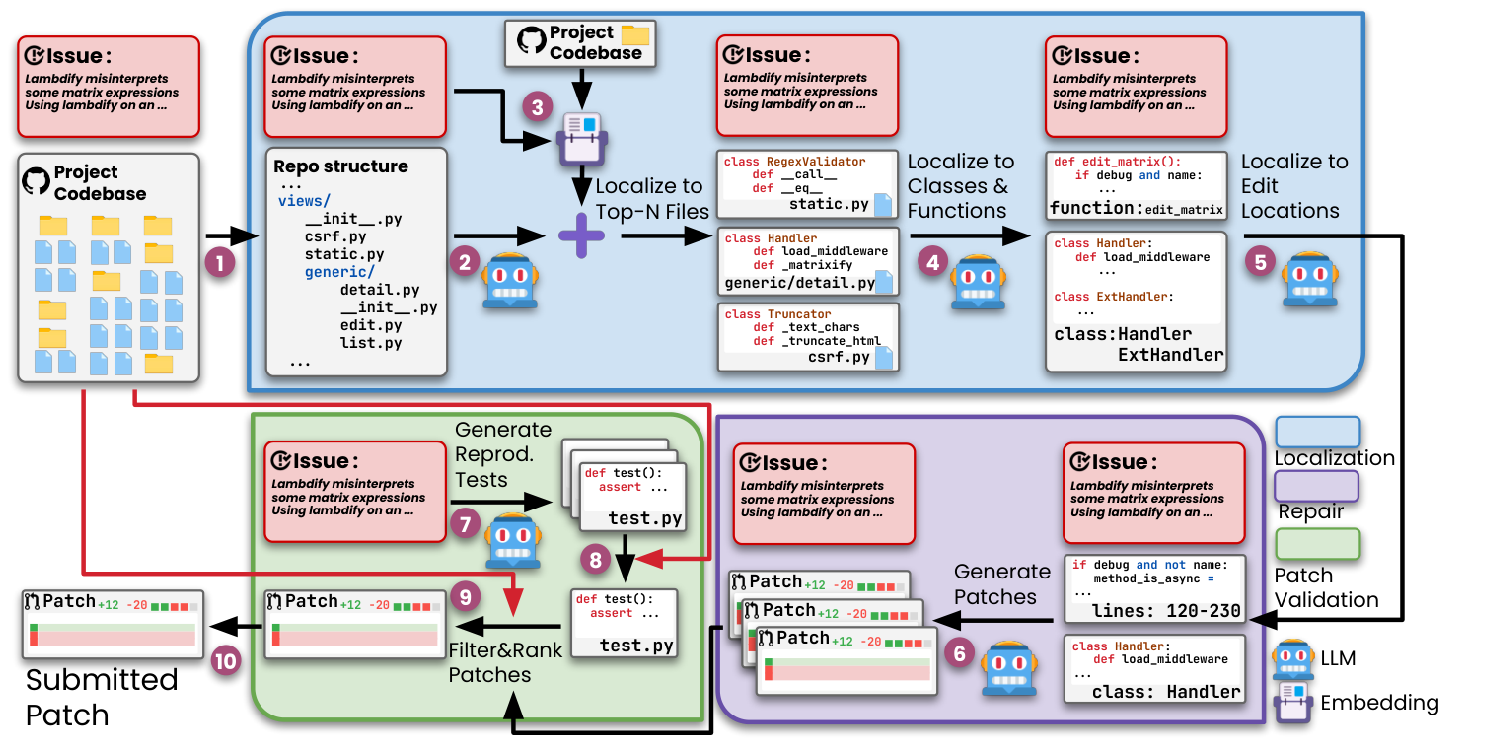
\includegraphics[width=\textwidth]{figures/Agentless分层定位修复与验证.pdf}
\caption{Agentless 将分层定位、补丁生成和验证过滤拆成固定阶段；下方验证区域同样使用复现测试。来源：官方课件第 37 页；对应口述 00:49:45--00:51:15。}
\end{figure}

讲者回顾，早期某些模型在这个工作流中比自由交互的 Agent 更有效：它们对单步代码任务训练充分，而工具调用及验证循环训练较少。这个观察说明，增加可选动作并不自动带来更好结果；执行方式需要与模型已学到的能力匹配。它也提醒读者，名称里的“Agentless”不能理解为整个系统从不执行代码。

\subsection{本章小结}
\begin{itemize}\setlength{\itemsep}{2pt}\setlength{\parsep}{0pt}\setlength{\topsep}{4pt}
\item 测试奖励可以训练单步代码模型；推理有助于形成正确且满足执行约束的实现。
\item DeepCoder 的训练响应预算扩展与 64K 评估扩展属于两个环节，曲线需按各自条件解读。
\item 仓库级 Agent 通过定位、编辑、验证反复缩小问题，验证还要覆盖相关回归行为。
\item 固定工作流同样可以包含多次模型调用与执行。有效性取决于工作流、模型和任务之间的配合。
\end{itemize}

\subsection{拓展阅读}
\begin{itemize}\setlength{\itemsep}{2pt}\setlength{\parsep}{0pt}\setlength{\topsep}{4pt}
\item \href{https://www.together.ai/blog/deepcoder}{DeepCoder 原始技术说明：测试奖励、响应预算与训练曲线}。
\item \href{https://arxiv.org/abs/2407.01489}{Xia 等：Agentless 的分层定位与固定修复工作流}。
\end{itemize}

\endgroup
\clearpage
\section{工具接口与代码定位}

定位、编辑和验证都需要通过工具落实。一个可运行命令的 Shell 已经能够完成很多操作；专用工具则能减少模型反复处理低层格式细节的负担。课程强调，工具接口与模型熟悉的输出形式会影响修复是否真正应用到文件，而定位方式还决定模型获得哪些上下文。

\subsection{一个 Shell 工具为何足以构成最小循环}

mini-SWE-agent 展示了一种简单设计：向模型提供运行 Shell 命令的接口。模型可以用 \texttt{rg}、\texttt{cat}、\texttt{find} 搜索和读取文件，用 \texttt{sed}、Python 或补丁命令修改文件，再运行 \texttt{pytest} 或构建命令检查结果。工具向模型返回输出、退出状态与超时情况，后续决策根据这些反馈继续进行。

\begin{figure}[H]
\centering
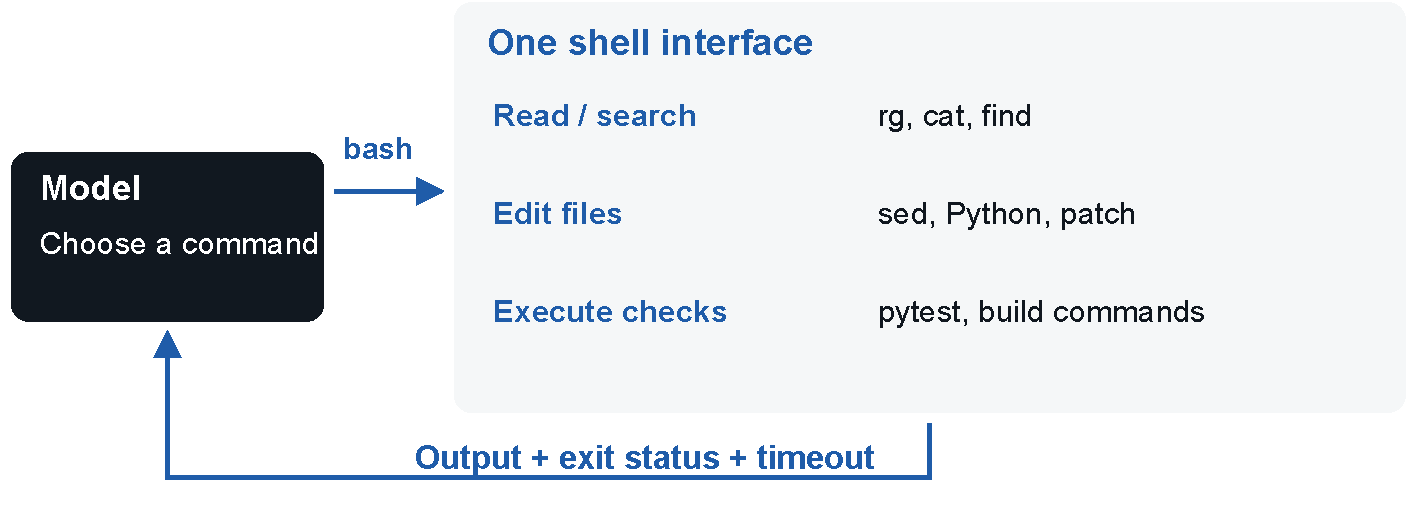
\includegraphics[width=.96\textwidth]{figures/Shell工具连接搜索编辑与执行.pdf}
\caption{单一 Shell 接口承载多种仓库操作；“只有一个工具”描述的是模型看到的接口数量。来源：官方课件第 39 页；对应口述 00:51:15--00:53:14。}
\end{figure}

这并不意味着只允许图中列出的几个命令。调试器等额外程序，也可以通过 Shell 调用。问题在于，模型每次编辑都需要选择命令、组织语法和转义；当许多调用都是文件操作时，这些负担会反复出现。

例如，课件用 \texttt{sed} 替换配置的一整行，再用新文件替换原文件。下面保留这一简单示例，假定文件中存在所示行。

\par\noindent\begin{minipage}{\textwidth}
\begin{lstlisting}[language=bash,caption={课件示例：通过 Shell 替换配置行}]
sed 's/^RETRIES = 3$/RETRIES = 5/' \
  settings.py > settings.new
mv settings.new settings.py
\end{lstlisting}
\end{minipage}

这种方式在简单文本上容易理解；遇到包含大量反斜杠、引号或复杂匹配的代码，模型还要正确处理 Shell 与编辑命令各自的规则。专用文件编辑工具把常见操作固定下来，让模型更集中地表达“改哪里、改成什么”。

\subsection{整文件、搜索替换与补丁格式}

整文件写入可以直接提供新的全部内容，易于应用；对较大文件而言，也要重复生成大量没有变化的代码，存在遗漏或意外改写的空间。搜索替换只发送旧片段与新片段，较为紧凑，但必须确认旧片段在当前文件中对应哪个位置。

\begin{figure}[H]
\centering
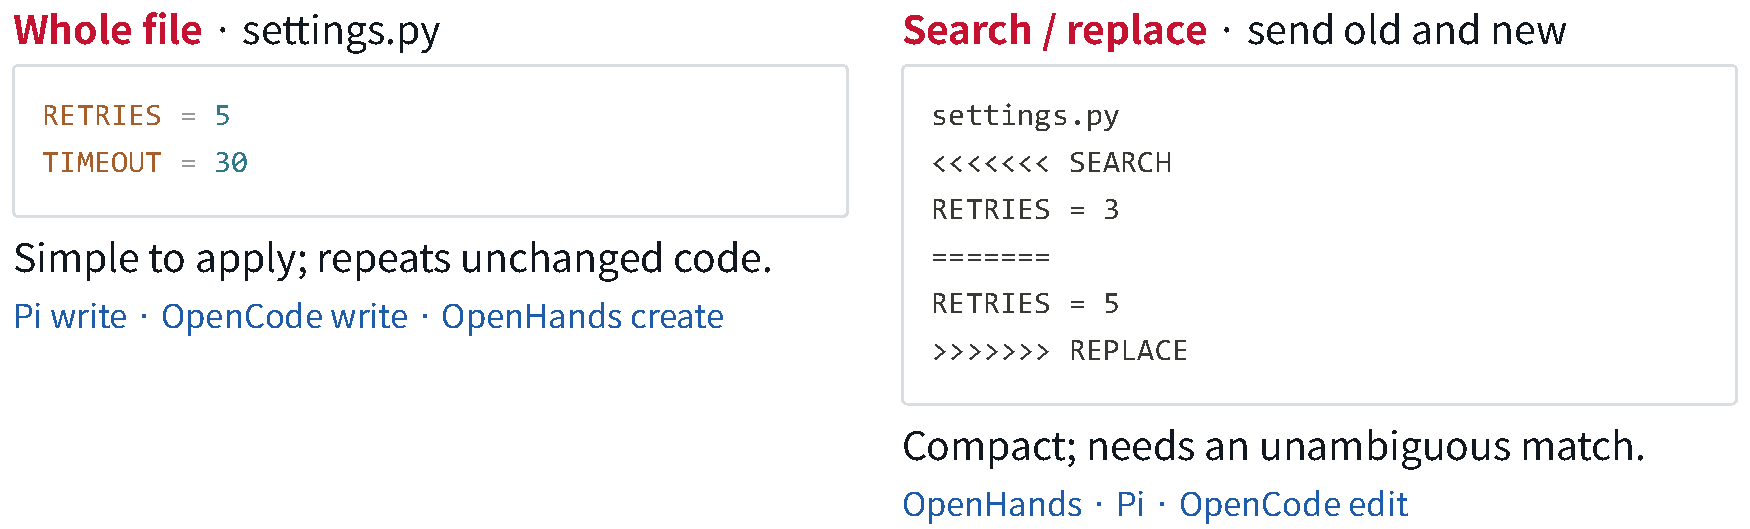
\includegraphics[width=\textwidth]{figures/整文件写入与搜索替换格式.pdf}
\caption{整文件写入重复未修改内容；搜索替换依靠旧片段的可辨识性。课件列出若干工具实现作为课程示例。来源：官方课件第 41 页；对应口述 00:54:38--00:55:26。}
\end{figure}

Unified diff 用 \texttt{---}、\texttt{+++} 标明文件，用 hunk 头给出位置及行数，并以 \texttt{-}、\texttt{+} 和上下文行表示删除、新增与保留内容。模型若填错行数或位置，会增加补丁应用的困难。因此，有些接口保留差分与上下文，却省去模型不易稳定生成的 hunk 行号；另一些接口使用显式文件操作标记，再用上下文定位。

\begin{figure}[H]
\centering
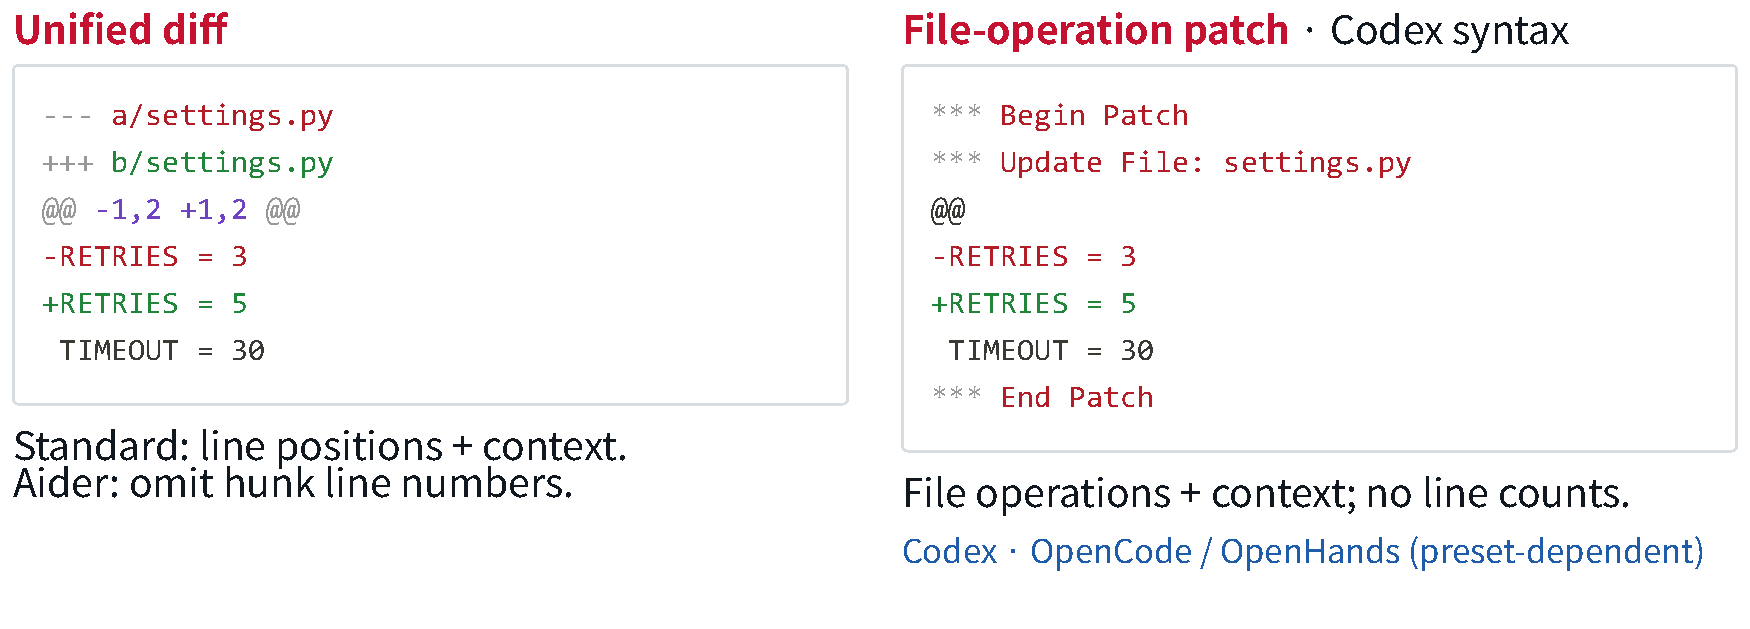
\includegraphics[width=\textwidth]{figures/UnifiedDiff与文件操作补丁格式.pdf}
\caption{左侧标准 Unified diff 给出行号和行数；右侧课件列出的文件操作补丁使用操作标记与上下文。两者有各自的解析协议。来源：官方课件第 42 页；对应口述 00:55:26--00:57:35。}
\end{figure}

\begin{warningbox}{省略行号后，仍然需要明确定位}
同一文件若有多处 \texttt{RETRIES = 3}，只提供这一行不足以判断应该修改哪一处。模型需要加入函数名、邻近行等上下文，并以工具的匹配结果确认应用位置。成功生成文本、工具接受修改、修改后行为正确，是三个相继要检查的状态。
\end{warningbox}

各种补丁格式服务于不同工具协议。图中的文件操作标记并非可直接交给标准 \texttt{patch} 命令的 Unified diff；编辑工具的具体校验、模糊匹配或拒绝策略，也取决于实现。课程以工具家族举例，不应据此假设所有版本和预设都共享完全相同的行为。

\subsection{接口改变为何能大幅影响结果}

课件引用 Aider 的历史重构实验：对 89 个 Python 任务，要求把大类中的方法移动为顶层函数，并检查代码是否保留和语法是否正确。使用 \texttt{gpt-4-1106-preview} 时，SEARCH/REPLACE 格式的成功率为 20\%，简化 Unified diff 格式为 61\%。

\begin{figure}[H]
\centering
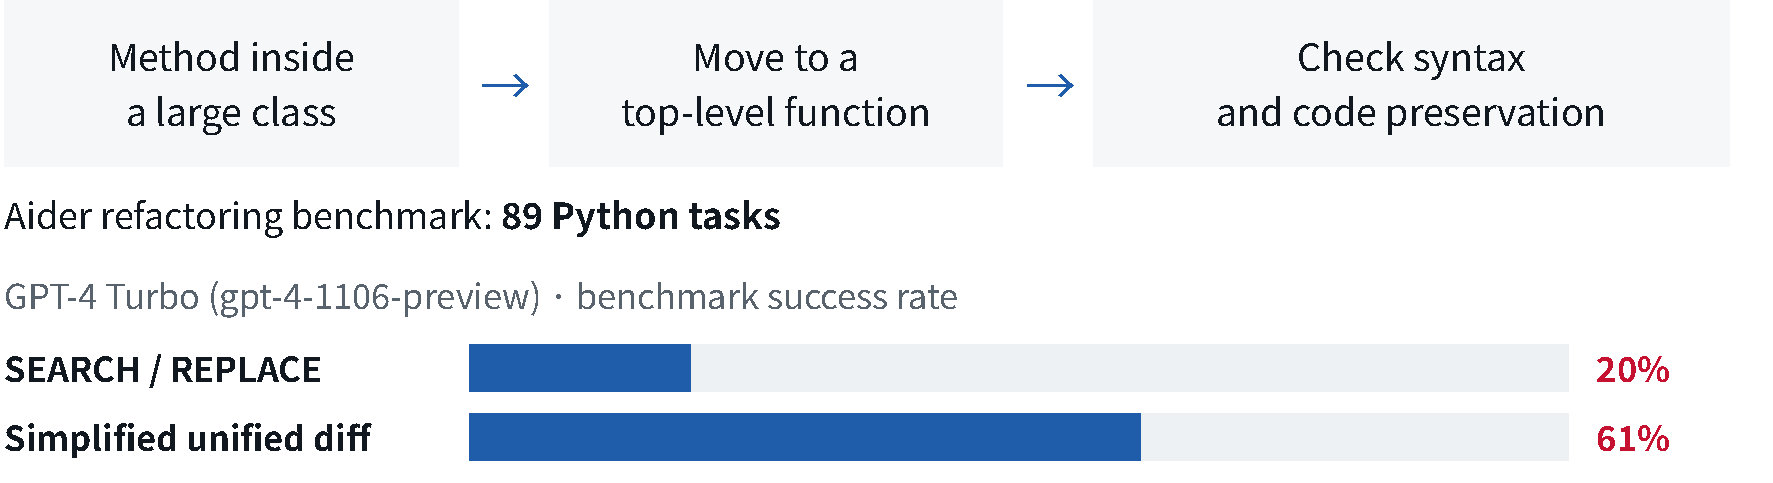
\includegraphics[width=\textwidth]{figures/Aider历史编辑格式重构实验.pdf}
\caption{同一历史模型和任务集上，改变编辑格式得到不同重构成功率；条件为 89 个 Python 任务、GPT-4 Turbo \texttt{gpt-4-1106-preview}。来源：官方课件第 43 页；对应口述 00:56:37--00:58:06。}
\end{figure}

讲者用模型在训练中对某种格式更熟悉来解释这种差异；Aider 原始说明同时讨论了格式设计与占位注释等失败问题。这个结果支持“接口是性能因素”，但不足以推导出简化 diff 对所有模型和所有编辑任务都优于搜索替换。模型与工具格式是否匹配，仍然需要在目标任务上观察。

\begin{importantbox}{工具接口参与了能力的表现}
模型对任务的理解需要转化成工具能接受的动作。接口决定模型要处理哪些格式、转义和定位细节；执行反馈决定它能否发现应用失败。评价一个编程 Agent 时，要把模型与工具协议共同看待。
\end{importantbox}

\subsection{从搜索症状到追踪相关依赖}

定位常从 Issue 中出现的名字、错误信息或行为开始。搜索 \texttt{retries} 可能同时得到命令行参数、配置读取函数和重试循环。出现匹配只能说明“与这个词有关”，不能直接说明“这里导致了错误”。接下来需要沿值的路径追踪：零最初在哪里被读入，默认值在哪里应用，又由哪些调用者消费结果。

LocAgent 是课程介绍的更结构化路线：构建代码依赖图，向 Agent 提供沿相关关系检索的工具。它可以从已找到的函数跳到调用者、使用结果的模块或关联测试，从而取得更有针对性的邻域上下文。

\begin{figure}[H]
\centering
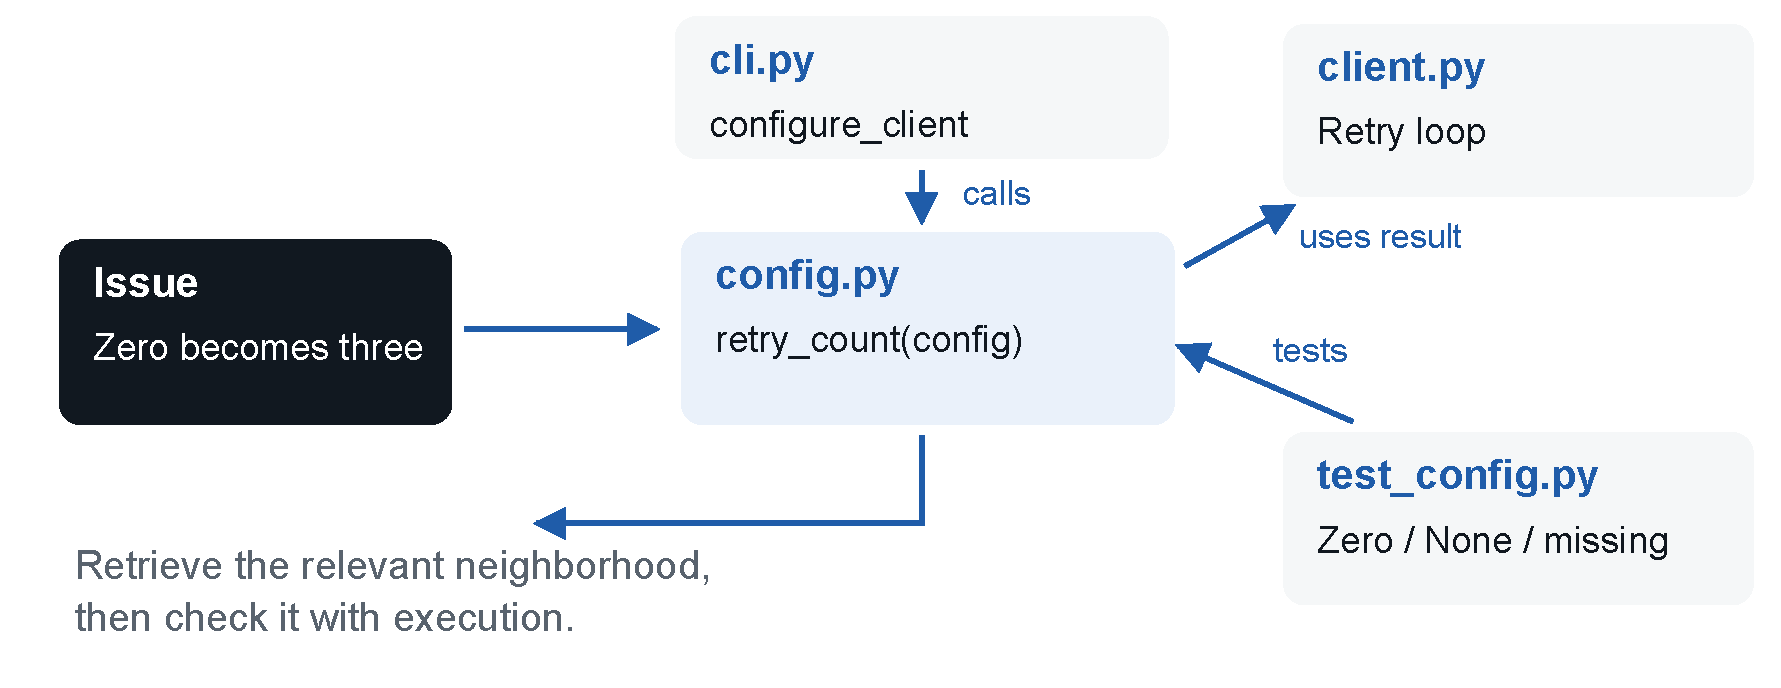
\includegraphics[width=\textwidth]{figures/依赖图辅助定位相关代码.pdf}
\caption{配置函数连接调用者、使用结果的重试循环与测试；相关邻域帮助形成修复范围，仍需执行验证。来源：官方课件第 45 页；对应口述 00:58:44--00:59:20。}
\end{figure}

依赖关系提供调查线索，但“与目标有关”不等于“存在缺陷”。作为教学补充，动态调用等机制也可能使静态图不完整。讲者在这一段末尾的经验判断是，更复杂的定位方法往往难以稳定超过简单搜索；这是对方法选择的提醒，不能当作否定依赖图检索的一般结论。下一部分将进一步讨论，怎样在仓库级任务上评价完整 Agent，并用可运行的任务训练它。

\subsection{本章小结}
\begin{itemize}
\item Shell 提供搜索、编辑与执行的通用途径；专用工具能减少重复的格式处理。
\item 整文件写入、搜索替换、标准 diff 与文件操作补丁具有不同成本和解析要求。
\item 历史编辑格式实验说明接口会影响成功率，结果需要保留模型、任务与格式条件。
\item 代码定位要从名称匹配推进到值与依赖关系的检查，并以执行结果验证修复假设。
\end{itemize}

\subsection{拓展阅读}
\begin{itemize}
\item \href{https://aider.chat/docs/unified-diffs.html}{Aider：编辑格式实验、简化 diff 与重构基准}。
\item \href{https://arxiv.org/abs/2503.09089}{Chen 等：LocAgent 的代码图与定位工具}。
\end{itemize}


\clearpage
\section{可执行任务：评价编程 Agent，也训练编程 Agent}

前面的定位、编辑和验证组成一次修复过程。接下来的问题是：怎样判断整个过程成功，怎样把大量这样的过程变成训练数据？课程在这里将评价与训练连接起来。一个包含起始仓库、明确问题和可靠检查的任务，既能评价 Agent，也能提供监督轨迹或强化学习奖励。

\subsection{SWE-bench：修好问题，同时保留已有行为}
SWE-bench 从真实 GitHub issue 及其相关修复中构造任务。Agent 得到问题描述和修复前的仓库状态，产出候选补丁；评价端把补丁及相关测试应用到对应仓库，再运行测试。参考补丁用于构建和核对任务，不应成为 Agent 的解题输入。

\begin{figure}[H]
\centering
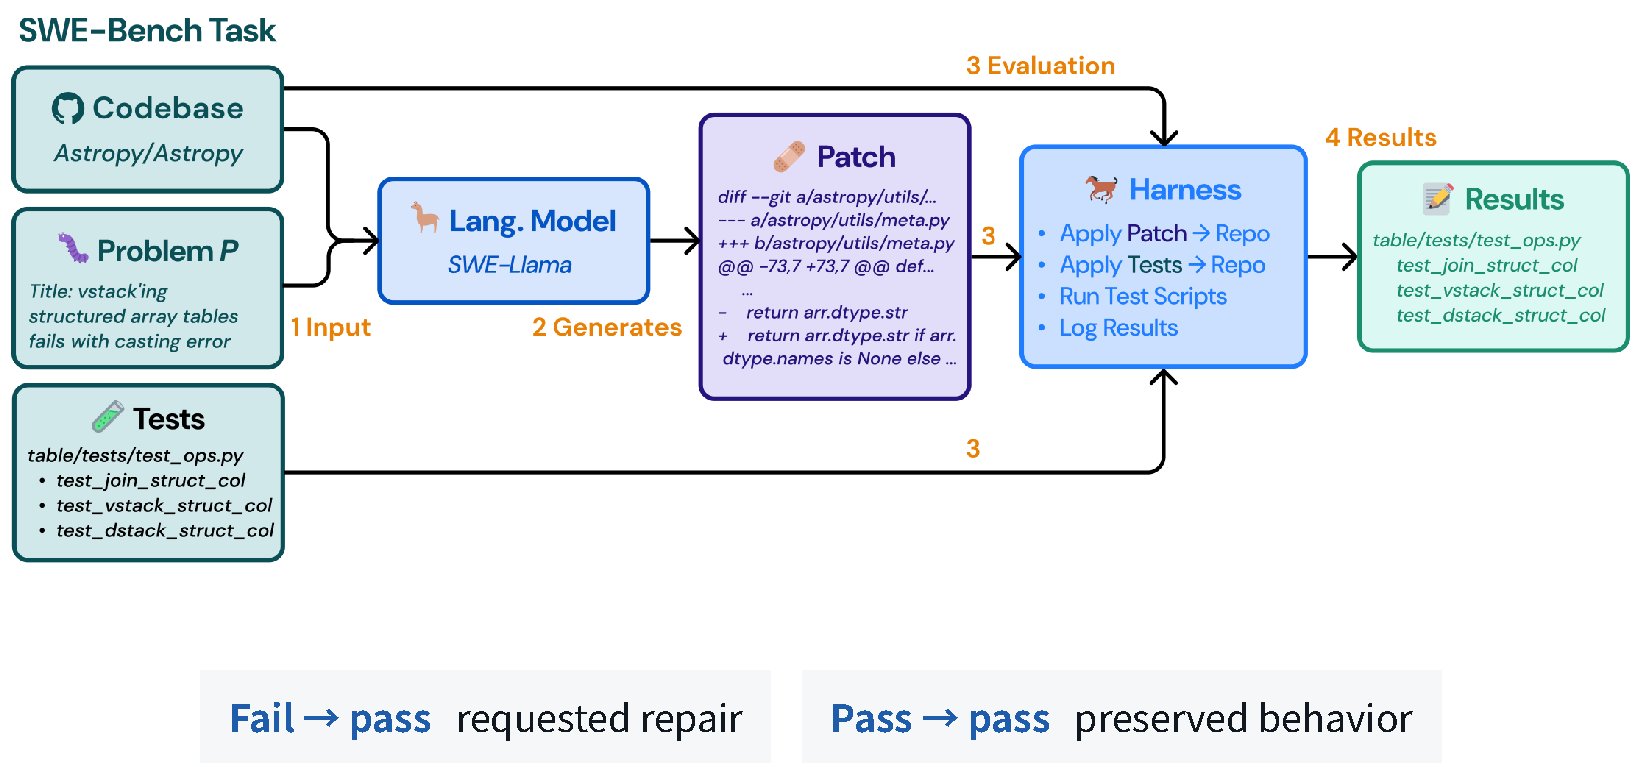
\includegraphics[width=\textwidth]{figures/SWE-bench补丁与测试评价流程.pdf}
\caption{仓库与问题进入模型，生成的补丁由评价环境应用并运行相关测试。图中的 Harness 指测试评价框架。\\{\footnotesize 来源：官方课件第 47 页；对应口述 00:59:20--01:02:00。}}
\end{figure}

为什么要分两组测试？只检查新功能，可能接受一个修好目标问题却破坏其他行为的补丁；把巨大仓库的所有测试每次全部运行，又可能显著增加成本。课程举例，一些大型项目的测试运行可能需要数分钟甚至更久。因此，基准选择相关测试来检查两类要求：
\begin{itemize}
\item \textbf{Fail $\rightarrow$ Pass}：修复前失败、正确修复后通过，检查本次 issue 要求恢复的行为。
\item \textbf{Pass $\rightarrow$ Pass}：修复前通过、修复后仍应通过，检查相关已有功能是否出现回归。
\end{itemize}

\begin{importantbox}{一个修复任务有两个成功条件}
目标缺陷被消除，相关既有行为被保留。检查两组测试可以提高判断质量，但它仍只覆盖被选中的行为；通过有限测试不等于证明整个程序在所有输入上正确。
\end{importantbox}

\begin{knowledgebox}{Harness 在本讲中有两种含义}
\textbf{Agent harness} 管理提示、工具、Agent 循环和上下文；\textbf{evaluation/test harness} 应用补丁、配置执行环境、运行测试并收集结果。SWE-bench 流程图里的 Harness 属于后者。两者可以协作，但承担的职责不同。
\end{knowledgebox}

\subsection{先证明任务可运行，再收集轨迹}
一个文字 issue 尚不足以组成可训练环境。官方课件将 runnable task 拆成三个部分：
\begin{enumerate}
\item \textbf{起始状态}：精确的代码版本、依赖与运行时，以及可用的测试命令。
\item \textbf{问题描述}：需要达到的行为，尽可能包含复现条件与必要背景。
\item \textbf{检查}：目标缺陷在修复前确实可复现，参考修复恢复该行为，并且相关回归检查可运行。
\end{enumerate}
如果依赖装不上，或测试本来就随机失败，后续奖励会把环境故障混入模型能力。验证环境应发生在大规模生成训练轨迹之前。SWE-Gym 的重要贡献正是为训练提供额外的可执行软件工程环境，而不只在已有评价任务上反复测分。

\subsection{多步强化学习：奖励作用于整条修复轨迹}
单步代码生成可以直接运行输出程序；编程 Agent 则要经历搜索、阅读、编辑、测试和结束等多个动作。终局测试结果对整条轨迹给出奖励。它鼓励成功修复，但最后一次失败并不能直接告诉我们究竟是定位错误、编辑错误，还是验证不足。

用课件中的目标式表达，就是让策略产生的修复轨迹获得更高的期望奖励：
$$
\max_{\theta}\;\mathbb{E}_{\tau\sim\pi_\theta}[R(\tau)].
$$
\begin{itemize}
\item $\theta$：待训练策略的参数。
\item $\pi_\theta$：决定下一步 Agent 动作的策略。
\item $\tau$：一次完整交互轨迹，包含 Agent 动作及环境返回的观察。
\item $R(\tau)$：轨迹的奖励，例如终局修复是否通过规定检查。
\item $\tau\sim\pi_\theta$：按当前策略与环境交互，采样一条轨迹。
\item $\mathbb{E}$：对采样轨迹求期望；$\max$ 表示选择参数以增大该期望。
\end{itemize}
官方第 49 页把 Assistant 的动作列为训练目标，而搜索结果、文件内容和测试输出提供后续决策的上下文。终局奖励由环境计算；模型要学习的是怎样产生更有效的动作序列。课件用 R2E-Gym 作为相关多步修复强化学习的参考。

\subsection{训练规模与推理规模分别提高什么}
SWE-Gym 的课件实验同时展示两种扩展方向。
\textbf{训练时扩展}增加用于训练的成功轨迹数量，改变模型参数；\textbf{推理时扩展}为同一任务生成多个 Agent rollout，再用学到的 verifier 选择候选，增加单次任务所用的计算。

\begin{figure}[H]
\centering
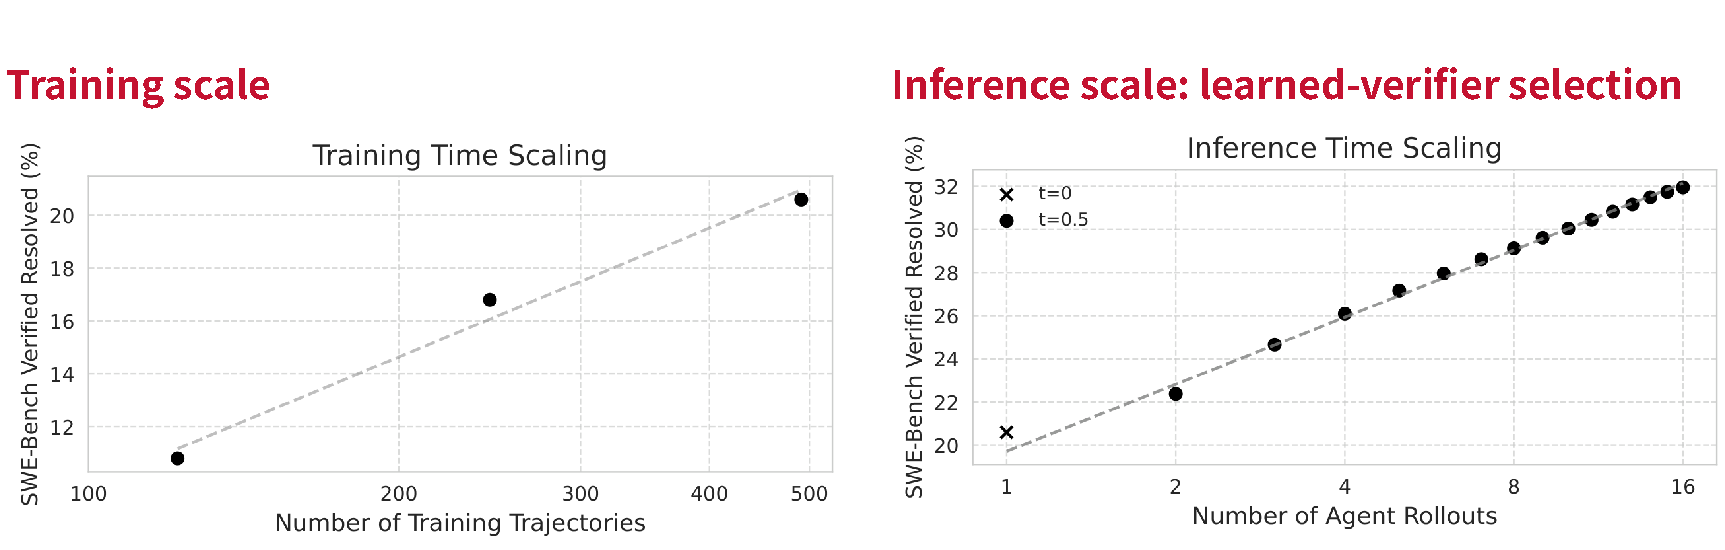
\includegraphics[width=\textwidth]{figures/SWE-Gym训练与推理计算量实验.pdf}
\caption{SWE-Gym 的 32B 模型实验：左图横轴为训练轨迹数量，右图为每任务 Agent rollout 数量，纵轴均为 SWE-bench Verified 解决率。\\{\footnotesize 来源：官方课件第 50 页；对应口述 01:03:19--01:04:10。}}
\end{figure}

左图从约 150 条训练轨迹、约 11\% 的解决率，增加到约 500 条轨迹、约 21\%；右图在给定模型及学习到的 verifier 条件下，随 rollout 数从 1 增加到 16，解决率从约 20\% 上升到约 32\%。这些数字来自图中这一组实验，不能直接外推到其他模型或仓库。

\begin{warningbox}{多候选只有配合选择机制，才成为可用结果}
右图采用 learned-verifier selection。它不等于知道所有候选真实答案后再选择的 oracle 指标，也不等于任意增加重试次数都能得到同样收益。候选多样性、选择器质量和新增计算成本都影响最终表现。
\end{warningbox}

讲师在 01:04:10--01:05:03 还补充了课件未列出的 \href{https://arxiv.org/abs/2505.20411}{SWE-rebench}：通过自动化流程持续从新的真实修复中收集可执行任务，扩充训练资源和较新的评价问题。课堂提到的数据时间范围与后续更新计划属于讲课时的介绍；理解这一工作的关键是持续收集、过滤和验证任务的机制。

\subsection{SWE-smith：从正常程序中注入可检测缺陷}
真实修复记录提供自然任务，但每个样本往往需要找到合适的 PR、代码版本和环境。SWE-smith 展示了另一条扩展路线：从能正常执行测试的仓库出发，改变代码，保留已有测试，筛选新出现测试失败的修改。

\begin{figure}[H]
\centering
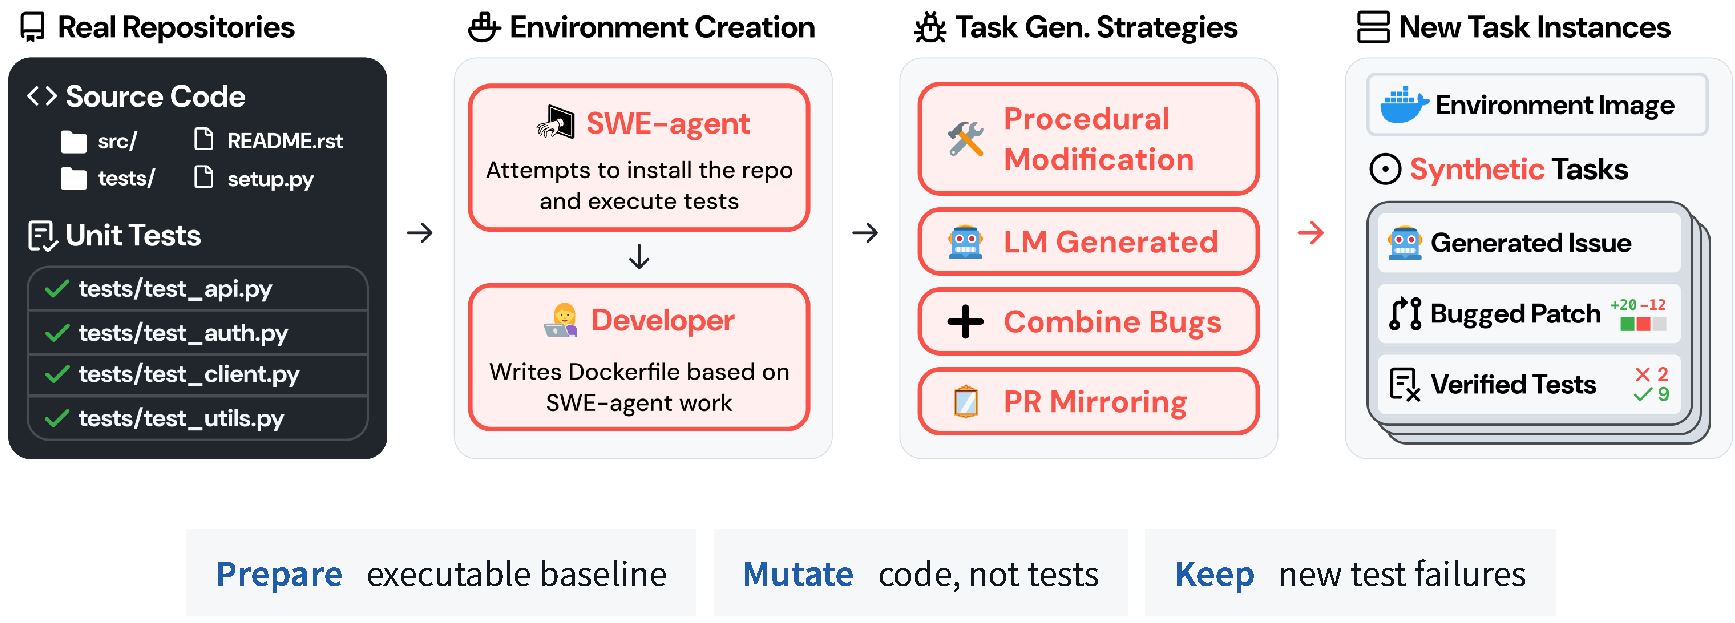
\includegraphics[width=\textwidth]{figures/SWE-smith注入缺陷构建任务.pdf}
\caption{SWE-smith 原始流程图包含环境构建及多种任务生成策略；课程重点说明准备可执行基线、修改代码并保留新增测试失败的路径。\\{\footnotesize 来源：官方课件第 51 页；对应口述 01:05:03--01:06:53。}}
\end{figure}

这与 mutation testing 有直接联系：人为制造应当改变行为的程序修改，再观察测试能否检测。一个 mutation 没有触发测试失败，可能说明测试未覆盖该差异，也可能说明它对所检查的行为没有影响，需进一步分析。用于修复任务生成时，已有测试检测到新缺陷，就提供了一个可验证的学习问题。

课件继续使用 retries 示例。原先仅在值为 \texttt{None} 时取默认值；把条件改成 \texttt{not value} 后，合法的零也被误当成缺省值。下面是依据课件第 52 页整理的教学对照：
\par\noindent\begin{minipage}{\textwidth}
\begin{lstlisting}[caption={同一行为的正常版本与注入缺陷版本（课件示例的教学整理）}]
def baseline(config):
    value = config.get("retries")
    return 3 if value is None else value

def mutated(config):
    value = config.get("retries")
    return 3 if not value else value
\end{lstlisting}
\end{minipage}

当输入为 \texttt{\{"retries": 0\}}，正常版本返回 0，变异版本返回 3。课件中的四项既有测试由全部通过变为三项通过、一项失败；恢复正确行为后再次全部通过。训练任务可据此要求 Agent 修复这一行为。

\begin{warningbox}{合成任务的可验证性与真实性需要分别检查}
注入缺陷便于增加任务数量，但缺陷类型、自然语言描述和真实开发需求的分布可能不同。通过合成样本训练后，应在保留的真实问题和新仓库上检查泛化能力。
\end{warningbox}

\subsection{多语言与多 Harness：让训练覆盖运行约定}
Multi-SWE-bench 与 SWE-bench Multilingual 把仓库修复扩展到多种语言。不同项目使用不同的依赖文件、构建命令和测试约定。课件举例，Python 常见 \texttt{pyproject.toml} 与 \texttt{pytest}，TypeScript 常见 \texttt{package.json} 与 \texttt{npm test}，Rust 使用 \texttt{Cargo.toml} 与 \texttt{cargo test}。这些是示例约定，具体命令应从项目配置中确定。

同样的模型在不同 Agent harness 中表现也可能不同。提示布局、文件编辑格式、工具返回格式和上下文管理都改变了模型面对的交互。多 Harness 训练让共享模型在多个真实接口下采样轨迹并获得奖励，从而减少对单一接口的依赖。

\begin{figure}[H]
\centering
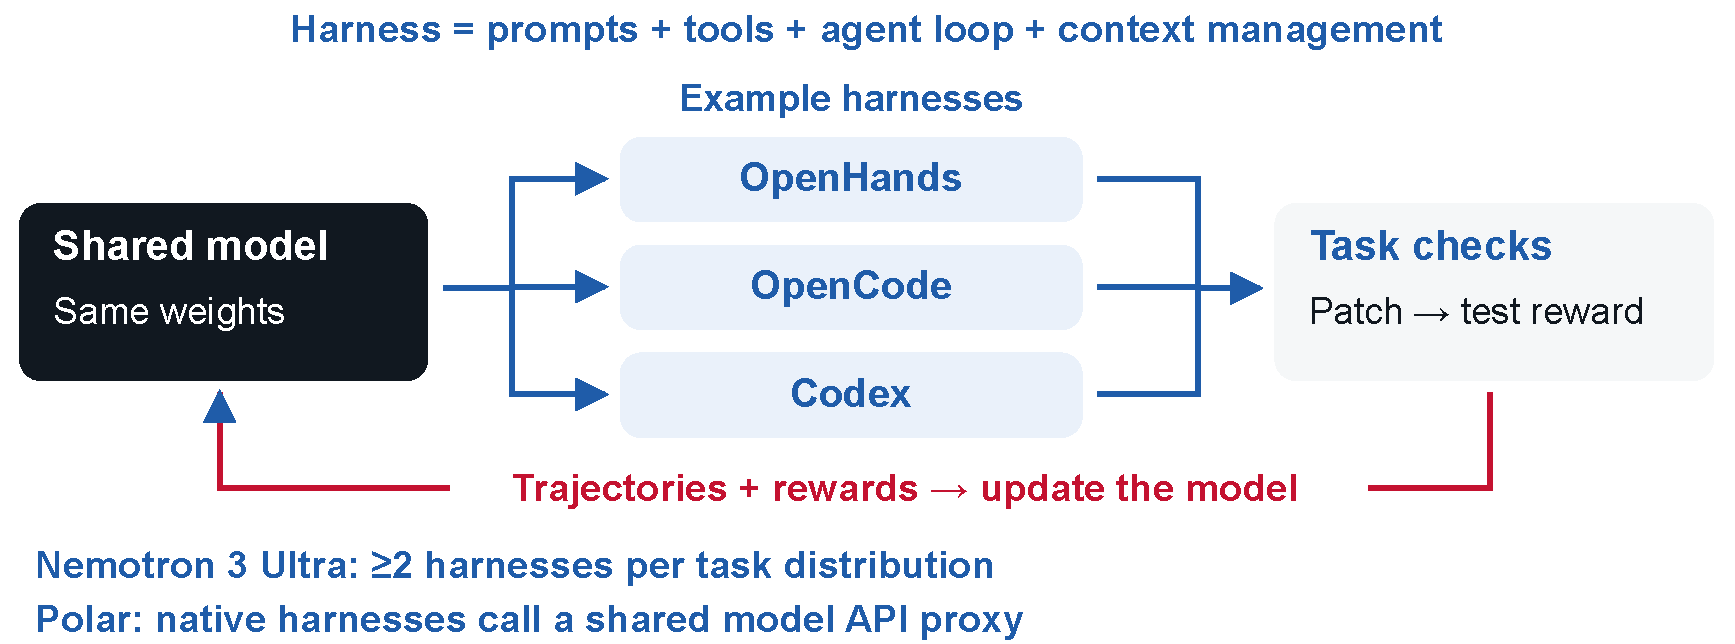
\includegraphics[width=\textwidth]{figures/共享模型的多Harness训练.pdf}
\caption{同一模型权重通过不同 Agent harness 执行任务；轨迹与任务检查奖励回流到训练。图中 OpenHands、OpenCode、Codex 为课件举例。\\{\footnotesize 来源：官方课件第 54 页；对应口述 01:08:04--01:09:19。}}
\end{figure}

官方课件列出 Nemotron 3 Ultra 在每个任务分布中使用至少两种 harness，以及 Polar 让原生 harness 调用共享模型 API 代理的方式。可迁移的原则是：\textbf{训练时的交互格式要覆盖实际使用时的交互格式}。不同工具名的堆叠本身，并不保证模型掌握其语义。

\subsection{本章小结}
可靠奖励建立在可靠环境之上。SWE-bench 检查目标修复与回归，SWE-Gym 提供训练环境，SWE-smith 扩展可验证合成任务。增加训练数据和增加推理 rollout 是两种不同的计算投入；多语言和多 Harness 则扩展模型能应对的运行约定。

\subsection{拓展阅读}
\begin{itemize}
\item \href{https://arxiv.org/abs/2412.21139}{Training Software Engineering Agents and Verifiers with SWE-Gym}：训练环境、轨迹与学习到的 verifier。
\item \href{https://arxiv.org/abs/2504.21798}{SWE-smith: Scaling Data for Software Engineering Agents}：环境建立与合成修复任务生成。
\end{itemize}

\clearpage
\section{前端开发：在浏览器中验证行为与呈现}

后端函数的输出常能直接用断言检查；前端还包含交互过程和最终页面。一个按钮可能调用正确函数，却无法点击；一个错误提示可能已写入 DOM，却被样式遮挡。因此，前端 Agent 仍沿用定位、编辑、验证循环，但验证需要进入浏览器。

\subsection{浏览器 Agent 与自动化脚本各自做什么}
课程给出两种方法。\textbf{浏览器 Agent} 逐步观察页面并选择下一次输入、点击等动作，适合需要根据状态继续探索的任务。\textbf{自动化脚本} 把动作和断言写成可重复执行的检查，例如用 Playwright 填表、点击、检查保存状态和截图。两种方法都可以获得页面图像，后续进行视觉检查或与经确认的基线比较。

\begin{figure}[H]
\centering
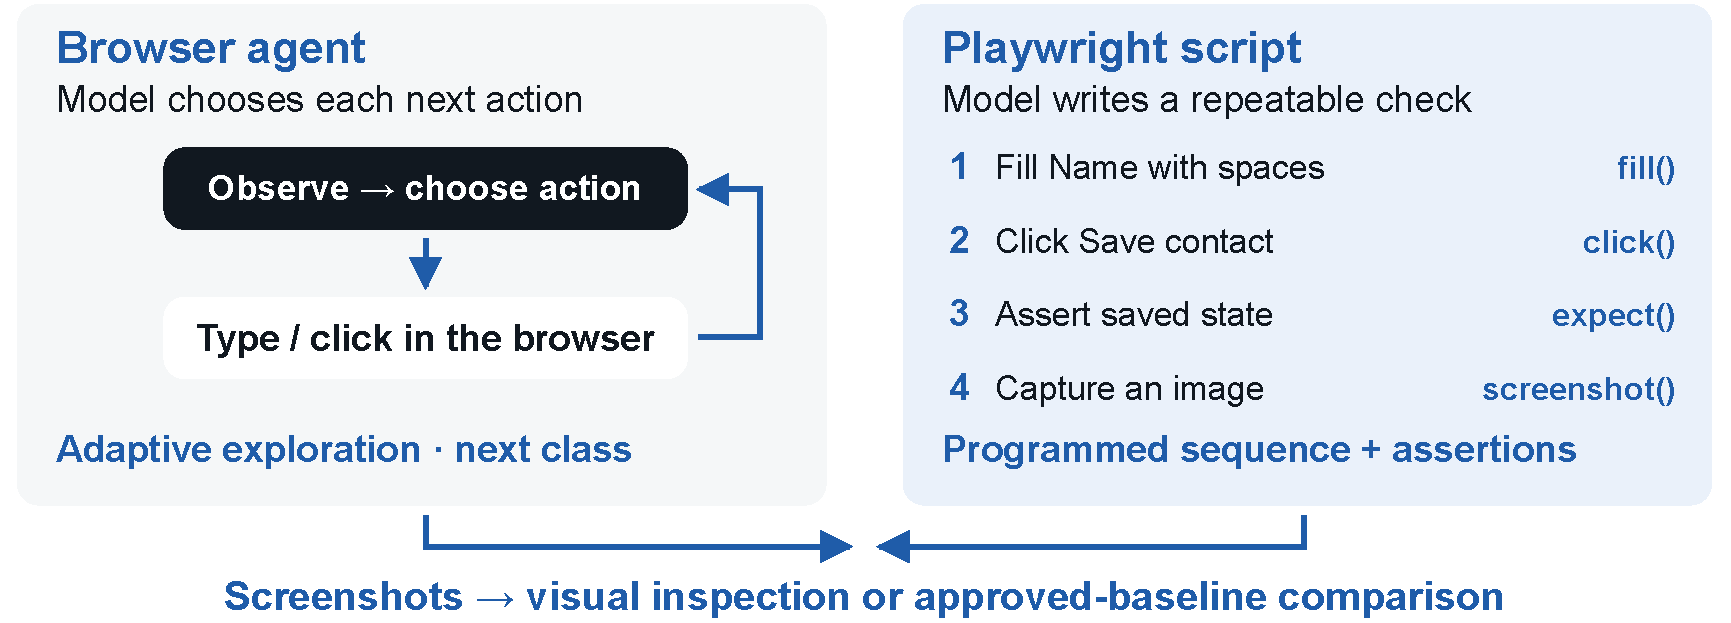
\includegraphics[width=\textwidth]{figures/浏览器Agent与可重复自动化脚本.pdf}
\caption{浏览器 Agent 逐步选择动作，Playwright 脚本执行预先写出的动作与断言；截图提供进一步的视觉检查材料。\\{\footnotesize 来源：官方课件第 57 页；对应口述 01:10:38--01:11:30。}}
\end{figure}

\subsection{一个空白姓名修复需要哪些证据}
课件的教学页面要求姓名至少包含一个非空白字符。旧逻辑只检查 \texttt{value.length}，一串空格长度大于零，因此可能错误保存一条记录。修改为检查 \texttt{value.trim().length}，可以检测这一输入。

\begin{figure}[H]
\centering
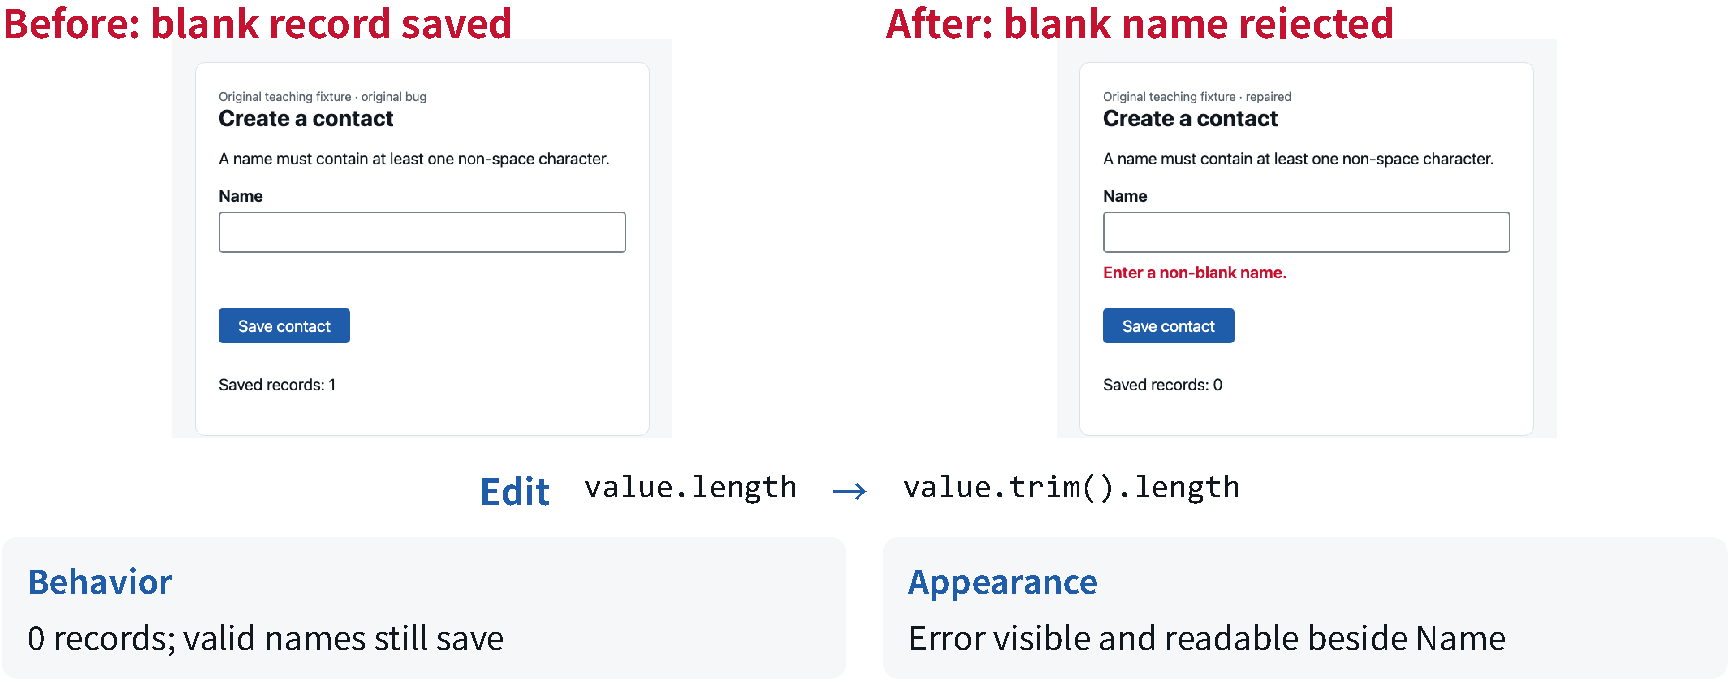
\includegraphics[width=\textwidth]{figures/空白姓名校验的浏览器修复前后.pdf}
\caption{课件示例：修复前保存了空白记录；修复后显示错误并保持零条记录。还要确认合法姓名仍然能保存。\\{\footnotesize 来源：官方课件第 58 页；对应口述 01:11:30--01:12:35。}}
\end{figure}

这里有三项分别需要检查的结果：空白姓名不能保存，正常姓名可以保存，错误提示在姓名附近可见且可读。下面将课件思路改写成 Python Playwright 教学测试；假设测试框架已提供 \texttt{page}，页面地址和可访问标签由具体应用确定。

\par\noindent\begin{minipage}{\textwidth}
\begin{lstlisting}[caption={空白姓名与合法姓名的浏览器行为检查（教学示例）}]
from playwright.sync_api import expect

def test_name_validation(page):
    page.goto("http://127.0.0.1:8000/contacts")
    name = page.get_by_label("Name")
    save = page.get_by_role("button", name="Save contact")
    name.fill("   ")
    save.click()
    expect(page.get_by_text("Enter a non-blank name.",
                           exact=True)).to_be_visible()
    expect(page.get_by_text("Saved records: 0",
                           exact=True)).to_be_visible()
    page.screenshot(path="blank-name-rejected.png")
    name.fill("Ada")
    save.click()
    expect(page.get_by_text("Saved records: 1",
                           exact=True)).to_be_visible()
\end{lstlisting}
\end{minipage}

断言检查保存状态和提示可见性，截图供检查具体呈现。单独保存截图没有自动完成视觉判断；若需要图像回归检查，还要定义可信基线、比较区域及可接受差异。

\subsection{SWE-bench Multimodal：图像输入与评分规则分开理解}
课程介绍 SWE-bench Multimodal 时强调，它主要评价视觉软件领域的\textbf{已有问题修复}，并非一般意义上从零设计前端。issue 可能包含图像来说明观察到的错误；Agent 需要据此理解要求，再修改起始仓库。

\begin{importantbox}{需求含图像，不能直接推导出图像相似度评分}
SWE-bench Multimodal 的补丁评价仍使用任务相关的执行测试与回归检查。截图帮助表达需求和检查页面，并不自动把最终评分变成“与参考图片越像越好”。先明确输入，再明确 verifier。
\end{importantbox}

讲师以不接收图像输入的 GLM-5.2 为例，提到它曾在前端设计 arena 上表现突出，这使他重新思考视觉能力对不同前端任务的作用。这个课堂观察可以说明：网页代码生成、带图 issue 理解、浏览器操作和视觉质量检查是不同能力。某一类偏好排名不能直接替代另外几类任务的评价；本讲仍认为视觉交互与检查是值得研究的组成部分。

\subsection{本章小结}
前端修复应同时检查交互行为和页面呈现。浏览器 Agent 提供自适应探索，自动化脚本提供重复性。图像可以进入需求和验证过程，具体评分仍由任务定义决定。GUI Agent 的构造方法将在下一讲展开。

\subsection{拓展阅读}
\begin{itemize}
\item \href{https://arxiv.org/abs/2410.03859}{SWE-bench Multimodal}：带视觉信息的软件问题与补丁评价。
\item \href{https://playwright.dev/python/docs/test-assertions}{Playwright 官方断言文档}：把页面行为转成可重复检查。
\end{itemize}

\clearpage
\section{更广的软件开发：任务、环境和时间跨度一起变化}

修复一个 issue 已经包含多个动作，但仍只是软件开发的一种任务。讲师在最后一段快速介绍定位、应用创建、整库实现、持续维护、测试生成和 CI 修复，指出它们对实际开发都重要，而训练数据与评价标准更难建立。

\subsection{实现内循环与开发外循环}
开发的内循环通常围绕编辑、调试和运行测试。外循环还包含需求澄清、代码审查、部署、监控以及维护。实现结果需要通过这些环节才能成为可持续使用的软件；不同环节要求不同证据。

\begin{figure}[H]
\centering
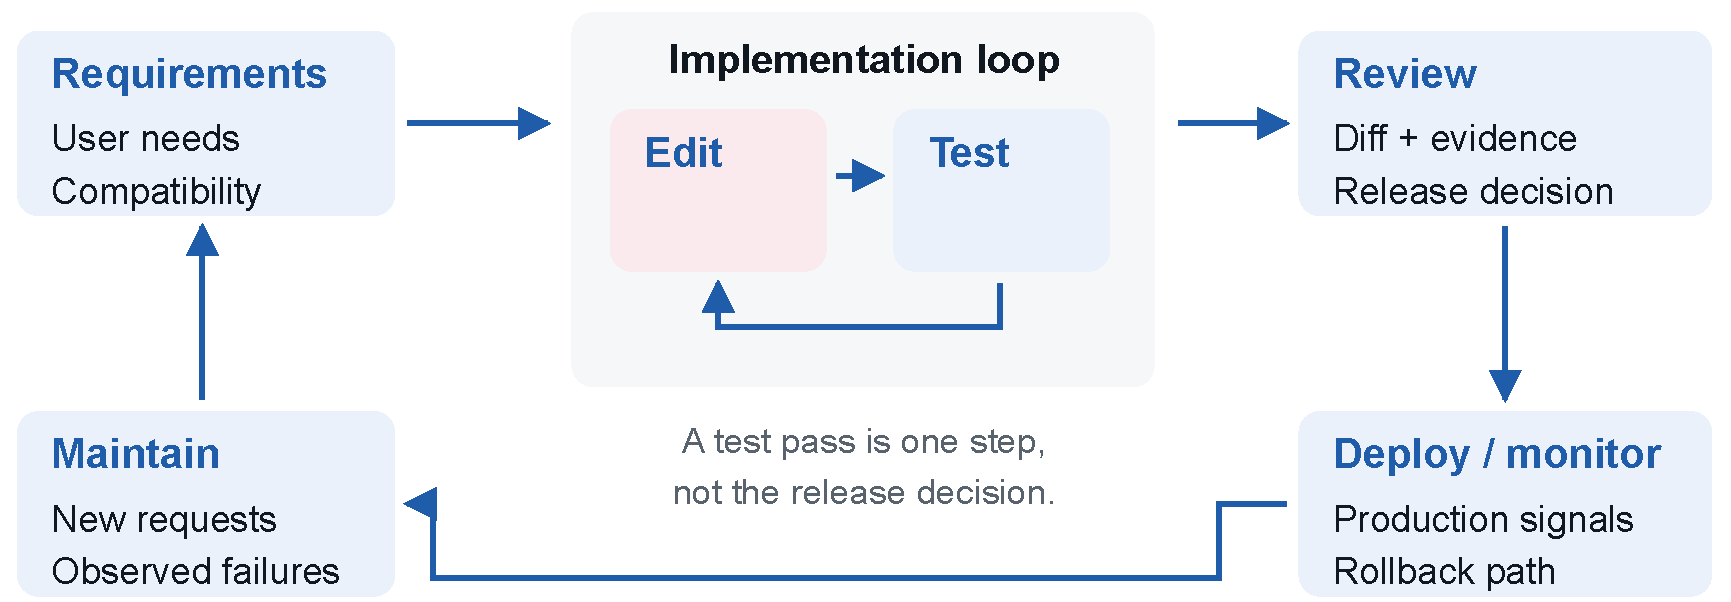
\includegraphics[width=\textwidth]{figures/软件开发的内层实现与外层流程.pdf}
\caption{需求进入实现循环，之后还需要审查、部署与监控；维护中的新请求和运行信号再次影响需求。\\{\footnotesize 来源：官方课件第 61 页；对应口述 01:12:35--01:14:10。}}
\end{figure}

为了说明任务覆盖的差距，课程引用 Microsoft 2019 年的开发者时间调查。官方课件第 62 页根据 5,928 个自报工作日整理：Coding 占 15\%，会议与邮件 25\%，调试及修复 14\%，运行测试 8\%，代码审查 5\%，其余还有需求与文档、帮助同事、学习等。

\begin{figure}[H]
\centering
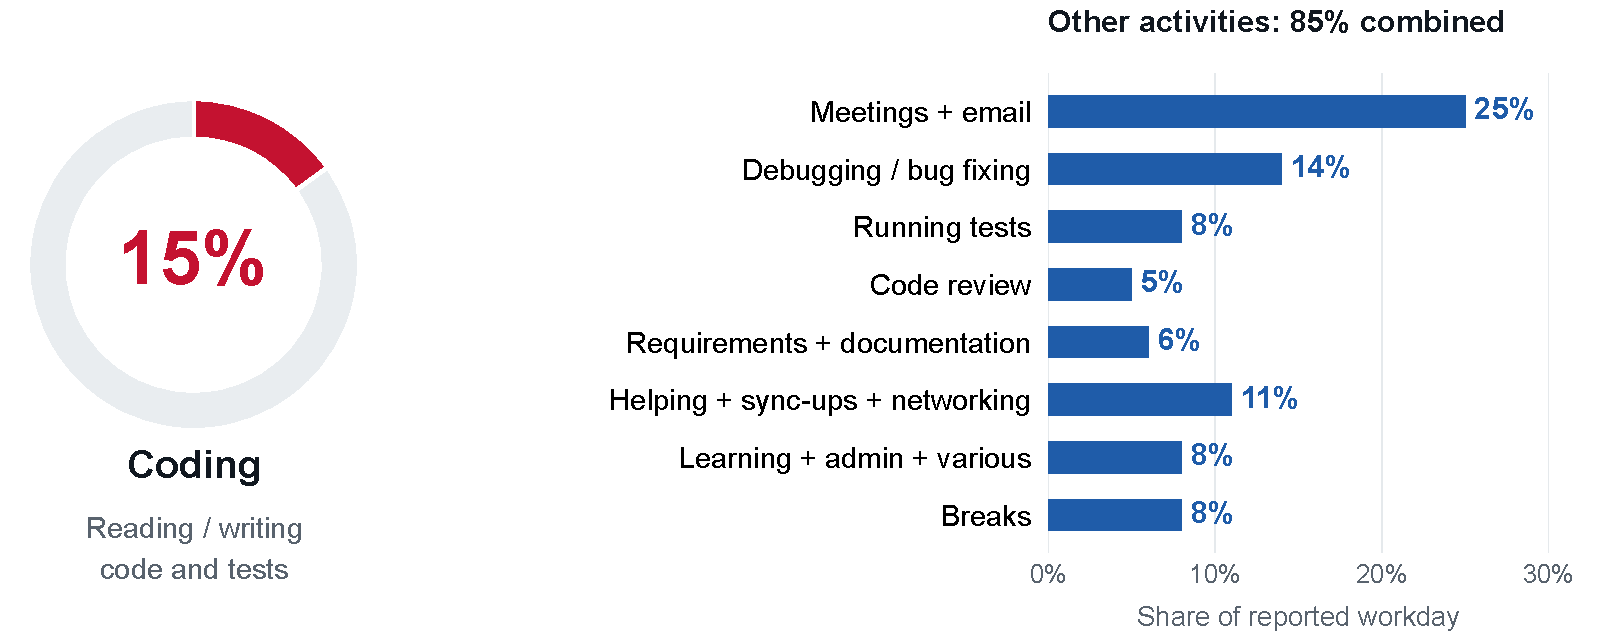
\includegraphics[width=\textwidth]{figures/Microsoft2019开发者时间调查.pdf}
\caption{2019 年 Microsoft 自报工作日调查：Coding 类别包括读写代码与测试，其余活动合计占 85\%。\\{\footnotesize 来源：官方课件第 62 页；对应口述 01:13:04--01:14:10。}}
\end{figure}

这一结果用于说明开发活动的多样性，不能解释成今天所有开发者都仅用 15\% 的时间写代码，也不能把剩余 85\% 直接当成 Agent 能节省的时间。


\subsection{按产物与验证环境区分任务}
官方课件第 63 页把开发任务放到同一张表里。比较它们时，需要同时观察产物、检查环境和任务跨度；同一个“成功率”名称可能代表很不相同的要求。
\begin{center}
\small
\begin{tabularx}{\textwidth}{L{2cm}L{2.6cm}XL{2.6cm}}
\toprule
任务 & 产物 & 环境与检查 & 时间跨度 \\
\midrule
Issue 修复 & 补丁 & 原仓库与相关回归测试 & 一个问题 \\
软件库创建 & 库实现 & 骨架、文档与包级测试 & 多个函数 \\
测试生成 & 新测试 & 对比缺陷版本与修复版本 & 一个目标行为 \\
CI 修复 & 代码或配置 & 工作流与必要构建检查 & 一次构建 \\
持续演进 & 累积改动 & 持续应用与里程碑、回归检查 & 相互依赖的任务 \\
\bottomrule
\end{tabularx}
\end{center}

\subsection{先拆出定位能力：CodeScout}
代码定位可以作为单独任务训练：输入 issue 和仓库，让模型搜索、阅读，输出相关文件、类或模块、函数等位置。CodeScout 用强化学习训练这种搜索策略；课件在文件、模块和函数三个粒度上，以参考修复位置计算 F1 奖励。参考补丁提供评分标签，不是策略输入。

将搜索能力独立出来，有助于研究较小模型、奖励设计以及工具使用。它也连接前面的经验：复杂仓库图或专用工具值得研究，但收益应与简单终端搜索比较。更丰富的工具接口不自动产生更有效的搜索策略。

\subsection{从创建应用到实现软件库}
\textbf{ViBench} 区分三类应用任务，课件记录的定义核对时间为 2026 年 9 月 7 日：Zero-to-One 从零创建应用（15 个应用）；Vibe-on-Ref 扩展参考 MVP（45 个）；Vibe-on-Vibe 扩展 Agent 先前创建的 MVP（45 个）。结果用人工编写的浏览器测试计划检查。三类任务分别测创建能力、对外部已有实现的修改能力和对自身先前设计的继续开发能力。

整库实现则要协调多个函数、模块和接口。课程对比 Commit0 与 ProgramBench：
\begin{itemize}
\item \textbf{Commit0}：得到库的骨架、文档和测试，补全实现，通过集成后的包级测试。
\item \textbf{ProgramBench}：面对参考可执行程序，通过输入探测观察输出，再从头实现能匹配可观察行为的程序。
\end{itemize}

\begin{figure}[H]
\centering
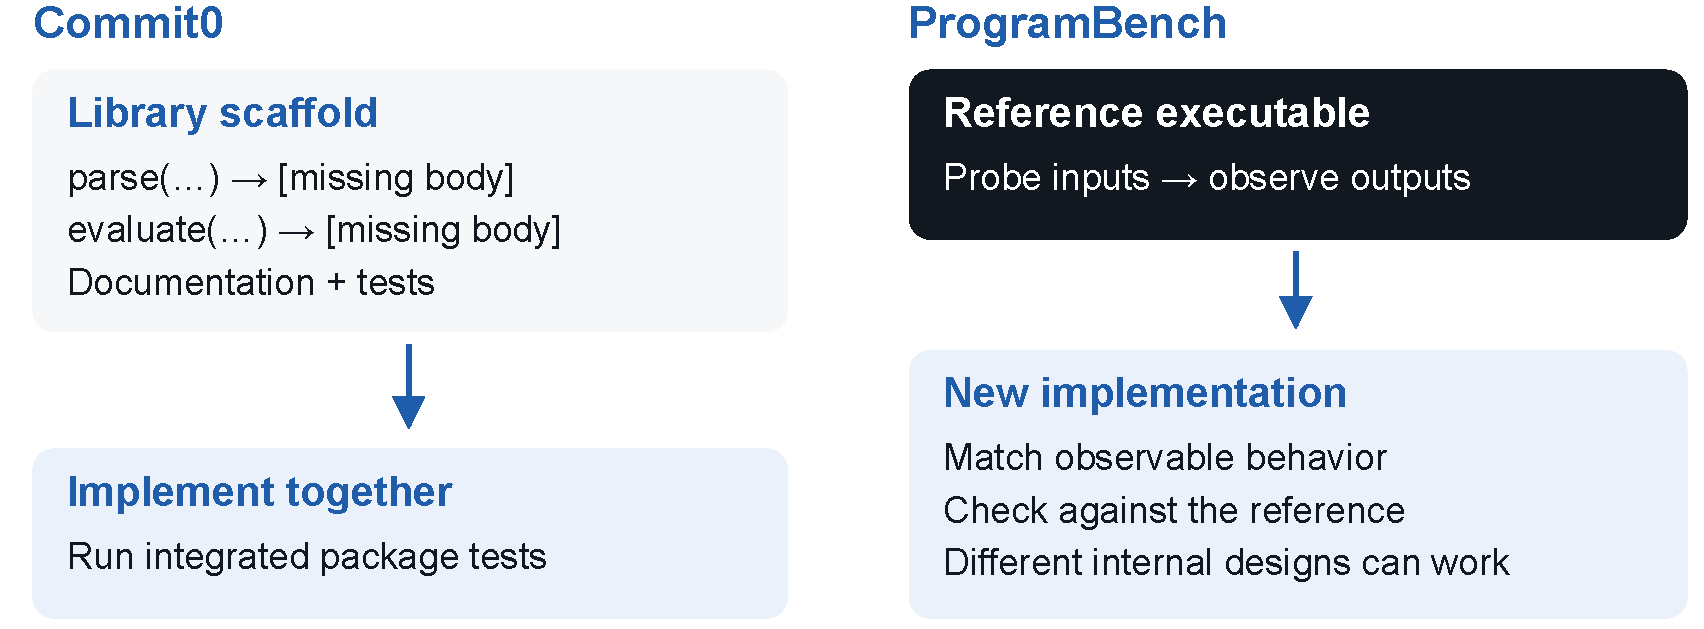
\includegraphics[width=\textwidth]{figures/Commit0与ProgramBench任务对比.pdf}
\caption{左侧通过骨架、文档和测试补全库；右侧通过参考可执行程序的输入输出行为指导重新实现。\\{\footnotesize 来源：官方课件第 66 页；对应口述 01:15:44--01:16:22。}}
\end{figure}

ProgramBench 不要求内部代码与参考实现相同；评价关心规定条件下的可观察行为。相比单函数任务，这类任务需要较长时间维持接口、状态和模块间的一致性。

\subsection{连续维护：前一项改动会成为后一项的起点}
SWE-Milestone 将独立 issue 扩展为有依赖的连续任务。Agent 的修改持续积累在同一代码库里，完成较早里程碑后再进入后续任务。第 67 页图中，M1、M2 完成后解锁 M3；每个里程碑都有相应检查。

\begin{figure}[H]
\centering
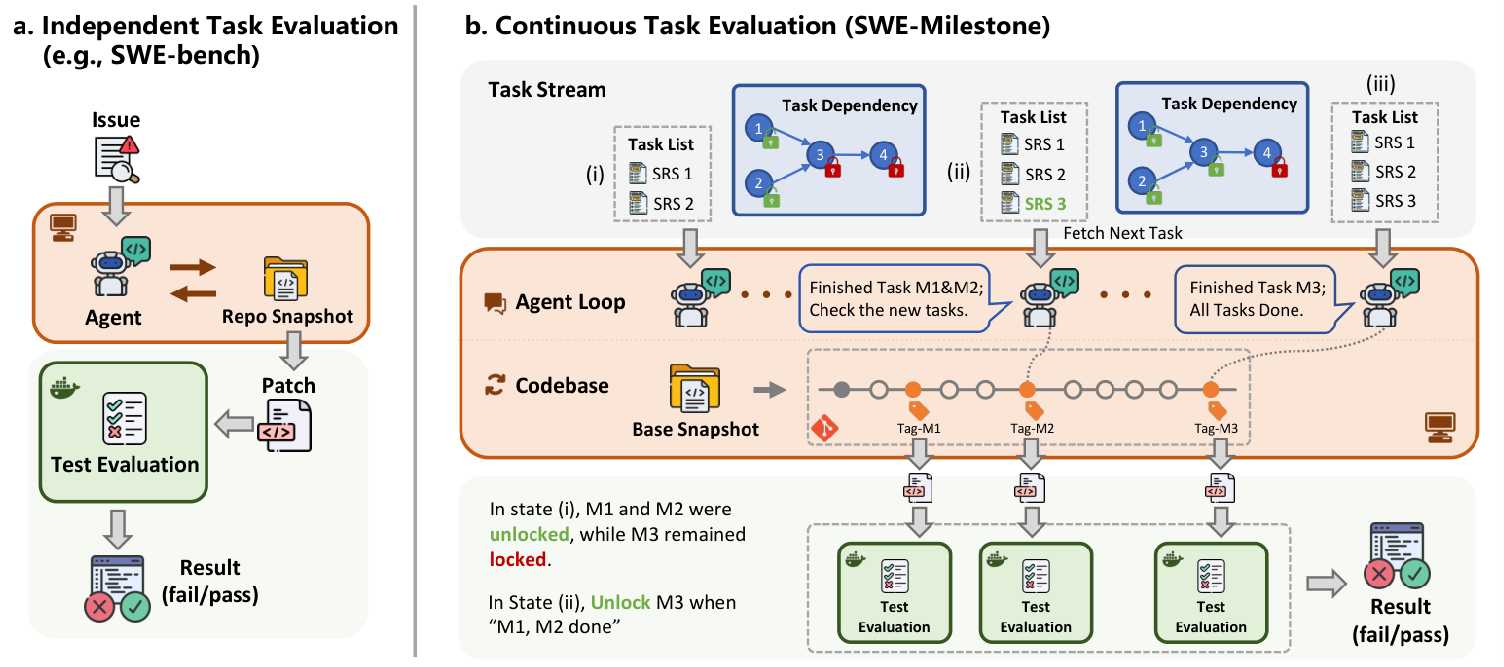
\includegraphics[width=\textwidth]{figures/SWE-Milestone连续任务与代码积累.pdf}
\caption{独立任务通常从各自仓库快照出发；连续任务保留已完成改动，并根据依赖解锁下一项任务。\\{\footnotesize 来源：官方课件第 67 页；对应口述 01:16:22--01:16:53。}}
\end{figure}

讲师强调，这类评价还需要关心代码是否越改越难维护。若一次修改用脆弱的特殊处理勉强通过，问题可能在后续任务才出现。因此，长时程评价能揭示单次修复分数未体现的累积成本。

\subsection{测试生成：让新测试区分缺陷与修复}
当产物由补丁改成测试，成功条件也随之变化。一个有针对性的缺陷复现测试，应该在有缺陷版本失败，在正确修复版本通过。只写出能运行的测试，还没有完成这一目标。

\begin{figure}[H]
\centering
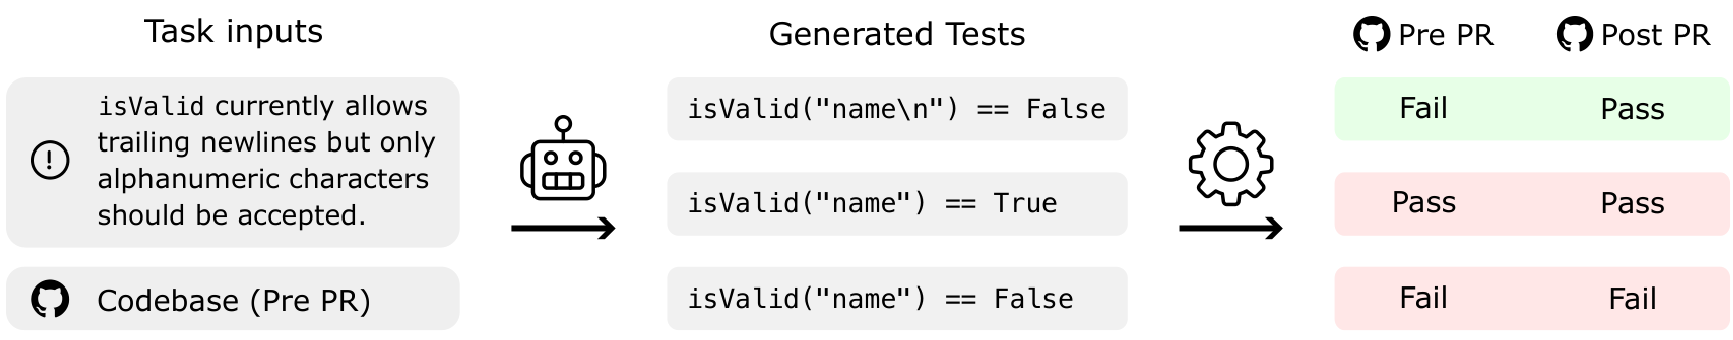
\includegraphics[width=\textwidth]{figures/生成测试区分修复前后行为.pdf}
\caption{SWT-Bench 的示例：拒绝尾随换行的检查在修复前失败、修复后通过；正常输入检查可能两边都通过；错误断言则可能两边都失败。\\{\footnotesize 来源：官方课件第 68 页；对应口述 01:16:53--01:17:27。}}
\end{figure}

图中 \texttt{isValid("name\textbackslash n") == False} 检测目标缺陷。\texttt{isValid("name") == True} 是合理的正常行为检查，但它单独不能证明发现了这次 bug；\texttt{isValid("name") == False} 在两个版本都失败，属于错误检查。mutation testing 还能衡量生成测试对注入缺陷的检测能力。

\begin{importantbox}{测试本身也是需要验证的程序}
检查测试能否执行、断言是否符合问题要求，以及能否区分有缺陷与正确修复版本。高质量测试把自然语言要求转为可执行反馈，随后 Agent 才能利用这个反馈反复改进补丁。
\end{importantbox}

\subsection{CI 修复：从运行日志追溯环境和配置}
CI 失败可能来自应用代码，也可能来自运行时、依赖、安装命令或工作流配置。课件第 69 页给出一个具体例子：工作流使用 Node 16，包声明需要 Node $\geq$18，\texttt{npm ci} 报 \texttt{EBADENGINE}。示例修复将运行时配置为 Node 20，并重新运行安装、构建和测试。

这个例子的判断顺序是：先从日志确定相关失败，核对项目支持的运行时，再改变与失败原因有关的配置。不能仅靠删除失败检查或放宽要求让工作流变绿。课件链接 JetBrains 的 LCA CI Builds Repair 数据；讲师同时指出，部署与运维任务需要实际基础设施，评价环境更难建立。

\subsection{训练可迁移技能：SWE-Playground 与 Hybrid-Gym}
课程最后简要提及两项工作，详细结构保留在官方课件中。\textbf{SWE-Playground} 自动提出项目和任务，建立仓库骨架与单元测试，实施并验证功能，再将项目用于多种能力的练习。

\begin{figure}[H]
\centering
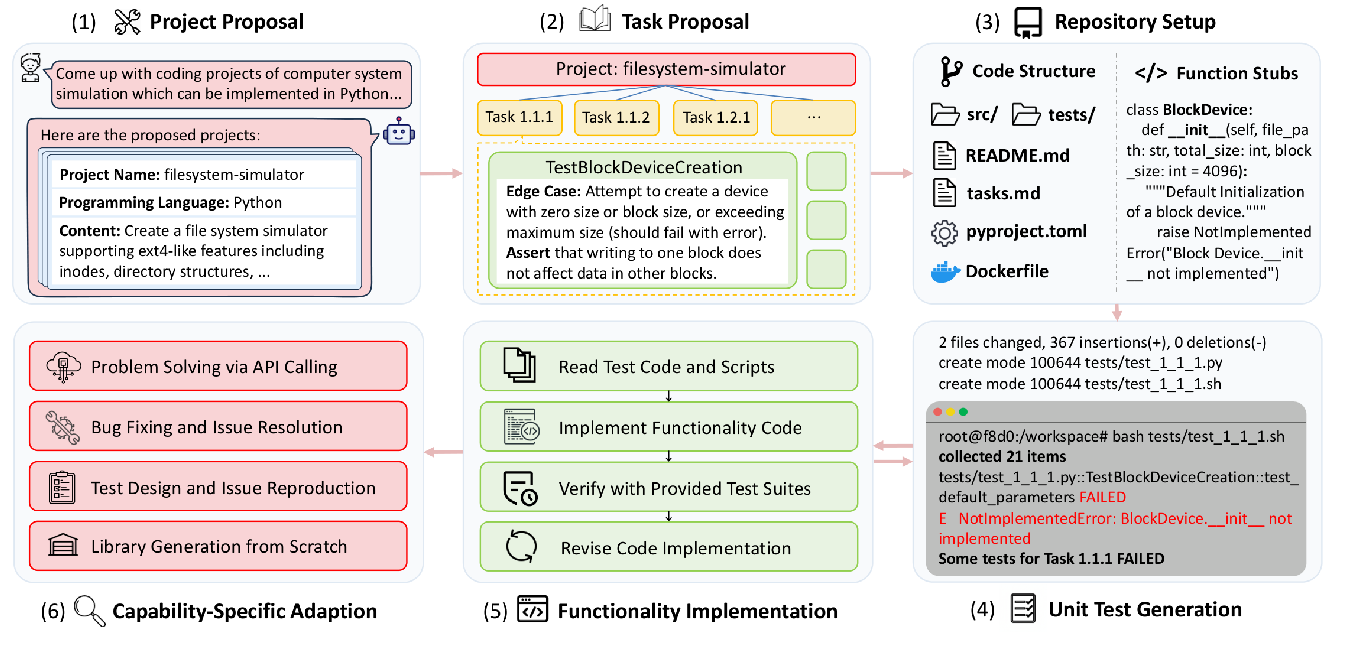
\includegraphics[width=\textwidth]{figures/SWE-Playground自动构建练习项目.pdf}
\caption{SWE-Playground 的六步流程：项目提议、任务提议、仓库建立、测试生成、功能实现和针对能力的任务适配。\\{\footnotesize 来源：官方课件第 71 页；课堂仅在 01:18:02--01:18:49 简要提及。}}
\end{figure}

\textbf{Hybrid-Gym} 研究不同开发任务共享的技能，例如定位函数、搜索依赖、理解规格以及构造检查。通过辅助任务训练策略，再在保留的新仓库与下游任务上检验迁移能力；比较时应控制推理预算。

\begin{figure}[H]
\centering
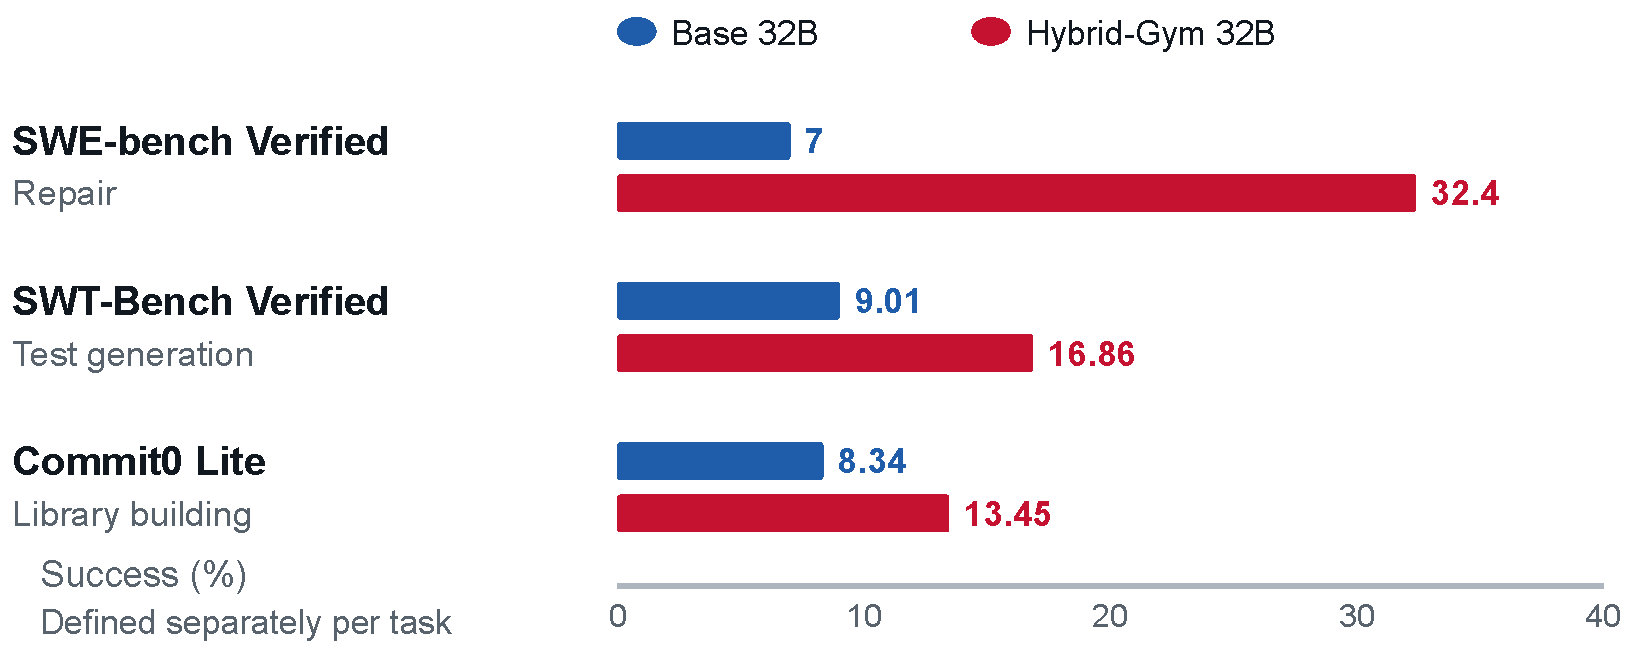
\includegraphics[width=\textwidth]{figures/Hybrid-Gym跨任务迁移实验.pdf}
\caption{课件选出的 32B 实验：修复、测试生成与库实现各自的成功比例均提高，但每个任务的成功定义分别确定。\\{\footnotesize 来源：官方课件第 72 页；课堂仅在 01:18:02--01:18:49 简要提及。}}
\end{figure}

课件记录的三组结果分别为 SWE-bench Verified 的 7\% $\rightarrow$ 32.4\%，SWT-Bench Verified 的 9.01\% $\rightarrow$ 16.86\%，Commit0 Lite 的 8.34\% $\rightarrow$ 13.45\%。这些结果支持在对应实验条件下存在技能迁移；由于各任务成功定义不同，不能把三个百分比视为同一个难度尺度，也不能由此断言所有开发任务都能同样迁移。

\subsection{本章小结}
软件开发任务同时改变产物、环境、验证方式和时间跨度。定位要找到相关位置，库实现要维持接口一致性，持续维护要承受累积改动，测试生成要区分缺陷，CI 修复要追溯运行条件。共享技能值得训练，收益要在未参与训练的任务和仓库上验证。

\subsection{拓展阅读}
\begin{itemize}
\item \href{https://arxiv.org/abs/2603.17829}{CodeScout}：面向代码搜索策略的强化学习。
\item \href{https://arxiv.org/abs/2602.16819}{Hybrid-Gym}：辅助技能训练与跨任务泛化。
\end{itemize}

\clearpage
\begingroup
\setlength{\parskip}{.2em}
\section{课件补充：代码行为预测}

\begin{knowledgebox}{本章的资料范围}
讲师在 01:18:02 开始的收尾段落明确说明时间已用尽，未能讲解 code world models。本章依据官方课件第 73--79 页及其原始参考资料整理，不代表视频中已经展开的口头讲解。
\end{knowledgebox}

\subsection{策略决定动作，世界模型预测动作的结果}
Agent 的策略回答“接下来做什么”；世界模型回答“如果执行这个动作，环境可能返回什么”。例如策略选择运行测试，真实环境实际运行后返回断言失败；世界模型则根据已有代码与工具历史，预测可能的测试输出。

可以把这两个条件分布并列写出，明确它们预测的对象不同：
$$
a\sim\pi(a\mid h),\qquad o\sim p(o\mid h,a).
$$
\begin{itemize}\setlength{\itemsep}{2pt}\setlength{\parsep}{0pt}\setlength{\topsep}{4pt}
\item $h$：已有交互历史，如已查看的代码与工具结果。
\item $a$：候选动作，例如运行测试或应用补丁。
\item $o$：执行动作后将观察到的环境结果。
\item $\pi(a\mid h)$：在历史条件下选择动作的策略分布。
\item $p(o\mid h,a)$：在历史及动作条件下预测结果的世界模型分布。
\item $\sim$：从相应分布采样；课件也允许使用预测结果来支持候选比较。
\end{itemize}

\begin{figure}[H]
\centering
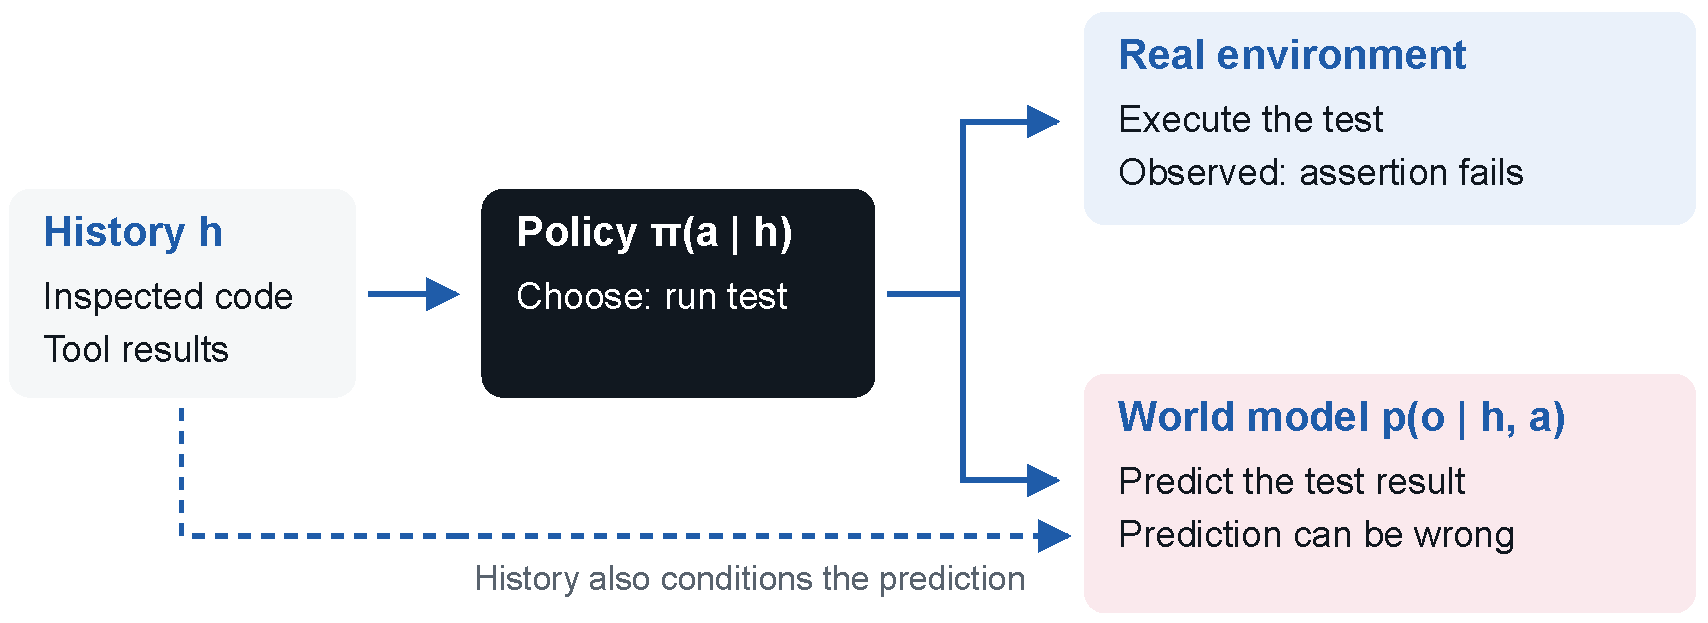
\includegraphics[width=\textwidth]{figures/策略选动作与世界模型预测结果.pdf}
\caption{历史同时影响动作选择和结果预测。真实执行获得观察，世界模型提供可能有误的预测。\\{\footnotesize 来源：官方课件第 74 页；未在本次视频中展开。}}
\end{figure}

\subsection{程序状态预测需要理解语义}
第 75 页用 Python 的共享引用说明错误预测的来源。下面直接整理课件中的代码：
\par\noindent\begin{minipage}{\textwidth}
\begin{lstlisting}[caption={共享引用会改变程序执行后的状态（官方课件第 75 页）}]
items = [1]
alias = items
alias.append(2)
result = len(items)
\end{lstlisting}
\end{minipage}

\texttt{alias = items} 让两个名字指向同一列表，没有复制列表。真实执行后 \texttt{items} 和 \texttt{alias} 都是 \texttt{[1, 2]}，\texttt{result} 等于 2。若模型把赋值误解成复制，就会预测错误状态。世界模型要学习的正是此类执行后果，而不只是生成语法上合理的代码。

\subsection{用预测筛选候选：收益与错误}
预测可以帮助筛选动作或补丁，但错误会改变 Agent 的决定。课件给出示意：A 是正确补丁，B 是错误补丁；模型预测 A 失败、B 通过，Agent 因此选择 B 并丢弃 A。

\begin{figure}[H]
\centering
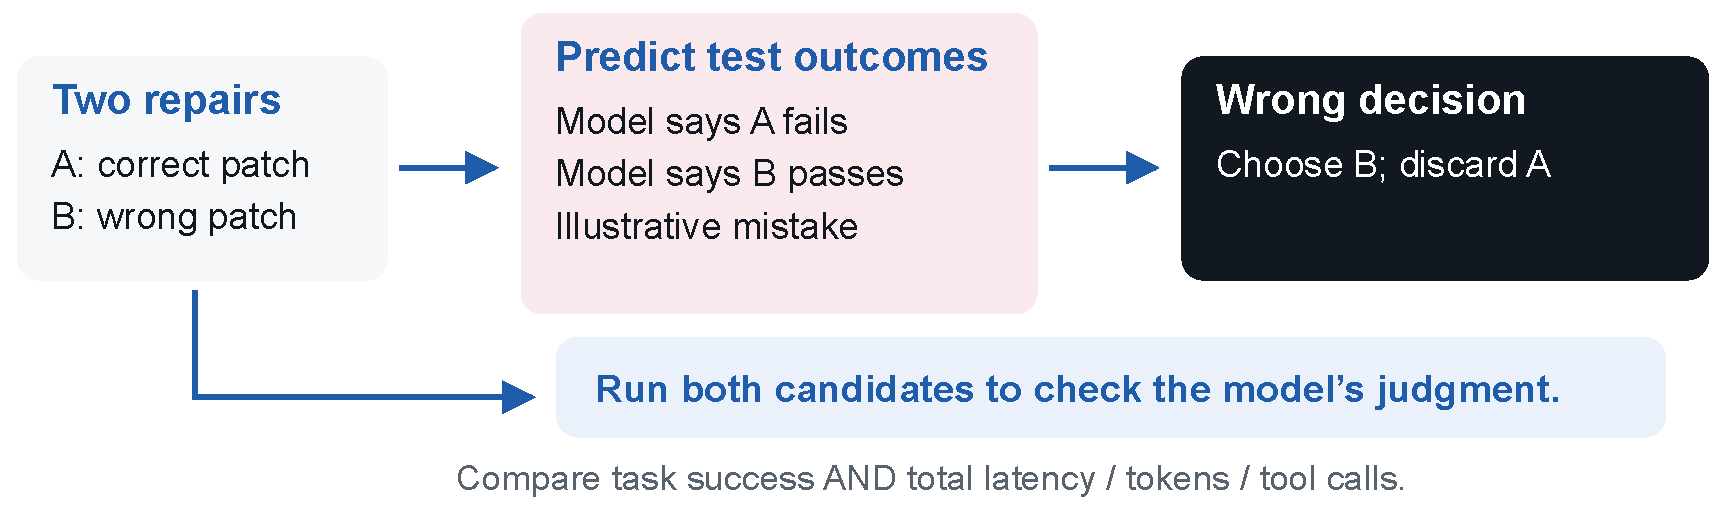
\includegraphics[width=\textwidth]{figures/错误预测如何误导补丁选择.pdf}
\caption{教学示意：错误的结果预测使候选选择发生反转；实际执行候选能够检查该判断。\\{\footnotesize 来源：官方课件第 76 页；未在本次视频中展开。}}
\end{figure}

因此，评价世界模型不能仅统计预测准确率，还要在同一组任务上检查最终任务成功率，以及总延迟、token 和真实工具调用次数。省去一部分运行，若导致更多错误修复，整体收益可能为负。

\subsection{两种路线：学会模拟执行，或生成可运行模拟器}
\textbf{CWM} 是学习计算环境行为的语言模型路线。官方课件引用 FAIR CodeGen 团队的工作：在通用预训练后，用 Python 解释器及 Agent 环境的观察--动作轨迹进行中期训练，之后进行监督微调及多任务强化学习。

\begin{figure}[H]
\centering
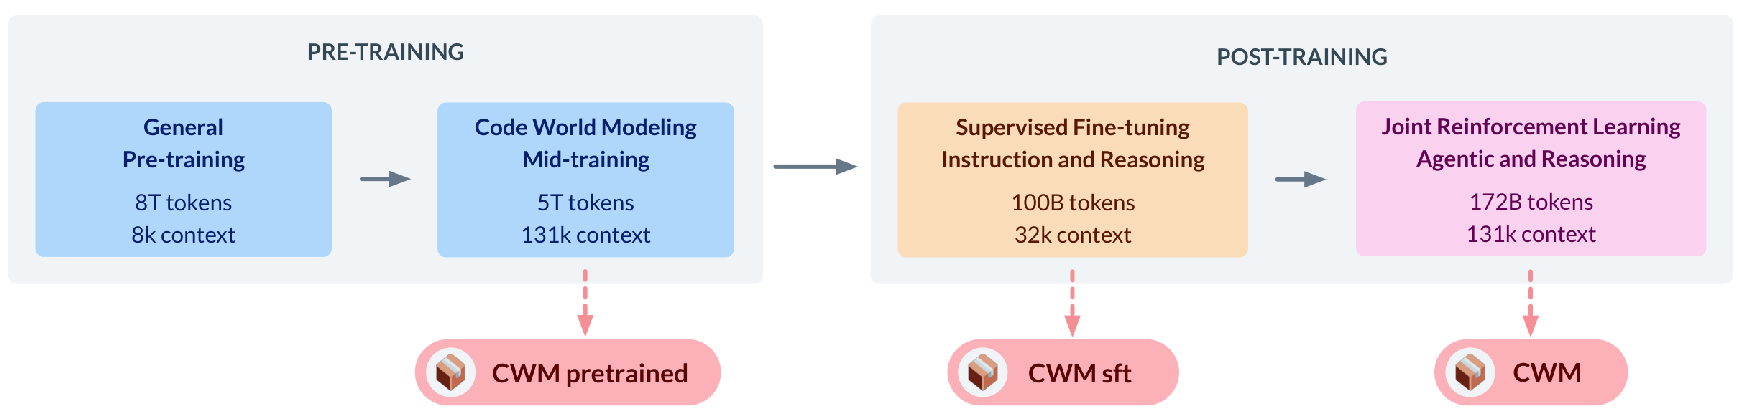
\includegraphics[width=\textwidth]{figures/CWM的分阶段训练流程.pdf}
\caption{CWM 原始训练流程：通用预训练、代码世界建模中期训练、指令与推理 SFT，以及 Agent 与推理的联合 RL。图中 token 数为各阶段训练量。\\{\footnotesize 来源：官方课件第 77 页；未在本次视频中展开。}}
\end{figure}

图中预训练与中期训练分别标为 8T 与 5T tokens，后续 SFT 与 RL 为 100B 与 172B tokens；上下文设置也随阶段改变。这里的 T、B 表示训练 token 数量级，不能当成模型参数量。研究报告中的 CWM 是 32B 参数模型。它为执行模拟、推理及规划提供研究基础，预测仍需通过实验检验。

\textbf{GIF-MCTS} 展示的是另一条路线：由 LLM 根据环境描述和已收集轨迹生成 Python 代码形式的世界模型，用实际环境轨迹校验其预测，再把错误反馈给生成、改进和修复过程。通过校验的代码模型可用于后续规划。

\begin{figure}[H]
\centering
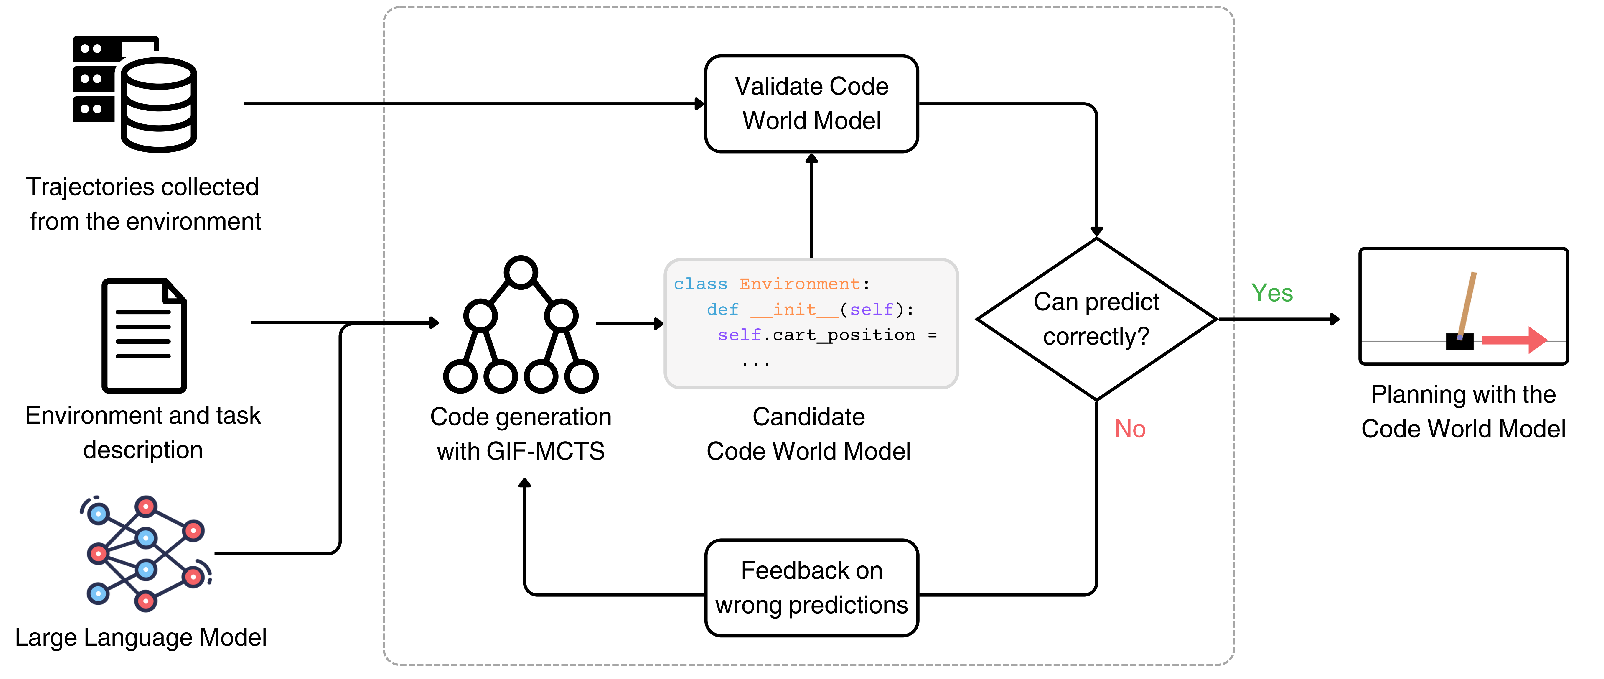
\includegraphics[width=\textwidth]{figures/GIF-MCTS生成并校验代码模拟器.pdf}
\caption{GIF-MCTS 构建代码模拟器：生成候选、用环境轨迹校验、根据错误继续改进，再用代码模型进行规划。\\{\footnotesize 来源：官方课件第 78 页；未在本次视频中展开。}}
\end{figure}

\begin{importantbox}{两种“代码世界模型”要按产物区分}
CWM 学习对计算环境后果的预测；GIF-MCTS 生成并校验一个用代码表达的模拟器。两者都服务于理解后果和规划，但模型形式、调用成本与错误来源并不相同。
\end{importantbox}

\subsection{课件留下的四个开放问题}
\begin{enumerate}\setlength{\itemsep}{2pt}\setlength{\parsep}{0pt}\setlength{\topsep}{4pt}
\item \textbf{决定是否变好}：在同一问题上，同时测预测错误与任务成功。
\item \textbf{总体是否更便宜}：计入预测自身的延迟和 token，以及真实环境调用。
\item \textbf{能否进入新环境}：保留未见过的程序、依赖和环境用于评价。
\item \textbf{何时回到真实执行}：改变回退阈值，既统计节省量，也统计失败。
\end{enumerate}
这些问题将代码预测与前面的验证循环重新接起来：预测可以支持决定，真实执行继续承担校验关键后果的职责。

\subsection{本章小结}
世界模型为动作选择提供后果预测，潜在收益是更好的搜索与更低的执行成本。收益取决于预测错误如何传导到任务结果；要把预测、候选选择、真实执行回退以及总成本放到同一评价中。

\subsection{拓展阅读}
\begin{itemize}\setlength{\itemsep}{2pt}\setlength{\parsep}{0pt}\setlength{\topsep}{4pt}
\item \href{https://arxiv.org/abs/2510.02387}{CWM: An Open-Weights LLM for Research on Code Generation with World Models}。
\item \href{https://arxiv.org/abs/2405.15383}{Generating Code World Models with Large Language Models Guided by Monte Carlo Tree Search}。
\end{itemize}

\endgroup
\clearpage
\begingroup
\setlength{\parskip}{.2em}
\section{总结与延伸}

\subsection{课堂结束时的重点}
视频末段把视野从单次 issue 修复扩大到实际软件开发：创建与维护应用、写测试、修 CI，以及训练可迁移的技能。讲师强调这些任务的重要性，也指出任务定义、训练数据和真实基础设施带来的困难。SWE-Playground 与 Hybrid-Gym 在收尾中被简要提及；代码世界模型因时间不足未展开。本讲的官方课件预告下一课为 Domains 2：GUI Agents，与前端部分的浏览器验证自然衔接。

\subsection{把本讲压缩为六个相互连接的问题}
官方课件第 81 页列出代码模型、Agent 编程、Agent 训练、前端开发、更广开发和代码行为预测六个方向。结合全文，可以用下面的教学归纳串起它们：
\begin{enumerate}\setlength{\itemsep}{2pt}\setlength{\parsep}{0pt}\setlength{\topsep}{4pt}
\item \textbf{模型从什么学到代码能力}：预训练提供代码与结构知识，中期训练对齐工作任务，执行反馈支持进一步强化学习。
\item \textbf{怎样把能力变为可完成的工作}：定位相关实现，使用匹配模型能力的编辑接口，再根据实际检查继续修改。
\item \textbf{怎样判断并训练这种工作能力}：可运行起始状态、清楚的要求与可靠检查共同形成任务；轨迹和奖励连接评价与训练。
\item \textbf{验证需要看到哪些后果}：后端关注执行结果，前端还要进入浏览器检查交互及呈现。
\item \textbf{任务能否延长和扩展}：多函数、连续维护、测试与 CI 要求不同 verifier；成功的一次修改还要能成为下一次修改的可靠起点。
\item \textbf{能否预先判断行动后果}：课件补充的世界模型可支持搜索与规划，价值应由实际任务表现和总成本确认。
\end{enumerate}

\begin{importantbox}{贯穿全讲的共同结构}
定义要达到的行为，提供可操作环境，让模型提出行动，再用与要求一致的反馈检查行动后果。模型、工具、任务和 verifier 必须彼此匹配，完整系统才会呈现稳定的开发能力。
\end{importantbox}

\subsection{最需要保留的判断边界}
\begin{itemize}\setlength{\itemsep}{2pt}\setlength{\parsep}{0pt}\setlength{\topsep}{4pt}
\item 代码外观、代码语义与可维护性需要不同证据，单一指标难以全部覆盖。
\item 测试通过的含义由测试覆盖范围、任务要求和执行环境共同限定。
\item 多次采样的收益同时依赖候选质量与选择方法，比较结果时应说明预算。
\item issue 图像、Agent 可用工具和评价规则分别定义，不能由其中一个推断另外两个。
\item 单次修复、持续开发和技能迁移回答不同问题，应分别设计保留任务与检查。
\item 预测执行后果带来节省的同时也可能误导决定，关键结果仍要有校验路径。
\end{itemize}

\subsection{本章小结}
本讲建立了从代码模型到软件开发系统的完整视角：学习代码、使用工具、定义任务、执行验证、扩展时间跨度，并研究预测能带来的帮助。沿着这条链条，最有价值的能力提升最终应表现为更可靠的任务完成，以及在相同条件下更合理的时间与计算成本。

\endgroup
\end{document}
